%%%% fatec-article.tex, 2024/03/10

%% Classe de documento
\documentclass[
  a4paper,%% Tamanho de papel: a4paper, letterpaper (^), etc.
  12pt,%% Tamanho de fonte: 10pt (^), 11pt, 12pt, etc.
  english,%% Idioma secundário (penúltimo) (>)
  brazilian,%% Idioma primário (último) (>)
]{article}

%% Pacotes utilizados
\usepackage[]{fatec-article}
\Author{1}{Name={ALMEIDA, Davi M.\\ VEIGA, Pedro X. \\ SILVA, Raphael P.\\ ARAI, Vinicius C.}}

\Author{2}{Name={\{ gilberto.satyro@fatec.sp.gov.br \}\\ \{ pedro.veiga01@fatec.sp.gov.br \} \\ \{ raphael.silva130@fatec.sp.gov.br\} \\ \{ vinicius.arai@fatec.sp.gov.br \}}}


%% Definição das palavras-chaves/keywords
\Keyword{1}{Trilha Pedagógica Gamificada}{Gamified Pedagogical Trail}
\Keyword{2}{RPG (Role-Playing Game)}{RPG (Role-Playing Game)}
\Keyword{3}{Metodologias Ativas de Aprendizagem}{Active Learning Methodologies}
\Keyword{4}{Educação Integral}{Integral Education}
\Keyword{5}{Gamificação Pedagógica}{Pedagogical Gamification}
\Keyword{6}{DUA – Desenho universal da Aprendizagem}{DUA – Universal Design of Learning}
\Keyword{7}{Tecnologia Educacional}{Educational technology}

%%%% Resumo no idioma primário (brazilian)
\begin{Abstract}[brazilian]%% Idioma (brazilian ou english)
  Este artigo propõe uma análise detalhada da aplicação de uma Trilha Pedagógica Gamificada com elementos de Role-Playing Game (RPG) no contexto educacional. A pesquisa visa desenvolver estratégias inovadoras baseadas em Metodologias Ativas de Aprendizagem, com o objetivo de promover um aprendizado mais significativo e inclusivo em qualquer ambiente acadêmico. O texto explora a relevância da Gamificação Pedagógica para engajar os estudantes, desenvolver habilidades e competências, e promover a construção do conhecimento de forma interdisciplinar. Além disso, discute a importância de alinhar essa abordagem com as diretrizes curriculares nacionais e os objetivos de uma educação integral. Por fim, são apresentadas reflexões sobre estudos da arte, metodologias similares e plataformas que realizam propostas semelhantes de gamificação pedagógica.
\end{Abstract}

%%%% Resumo no idioma secundário (english)
\begin{Abstract}[english]%% Idioma (brazilian ou english)
This article proposes a detailed analysis of the implementation of a Gamified Pedagogical Trail with elements of Role-Playing Game (RPG) in the educational context. The research aims to develop innovative strategies based on Active Learning Methodologies, with the goal of promoting more meaningful and inclusive learning in any academic environment. The text explores the relevance of Pedagogical Gamification to engage students, develop skills and competencies, and promote interdisciplinary knowledge construction. Additionally, it discusses the importance of aligning this approach with national curriculum guidelines and the objectives of a holistic education. Finally, reflections on state-of-the-art studies, similar methodologies, and platforms that propose 
similar pedagogical gamification approaches are presented
\end{Abstract}

%% Processamento de entradas (itens) do índice remissivo (makeindex)
\makeindex%

%% Arquivo(s) de referências
\addbibresource{fatec-article.bib}

%% Início do documento
\begin{document}

% Seções e subseções
%\section{Título de Seção Primária}%

%\subsection{Título de Seção Secundária}%

%\subsubsection{Título de Seção Terciária}%

%\paragraph{Título de seção quaternária}%

%\subparagraph{Título de seção quinária}%

\section*{Introdução}%
\label{sect:intro}
No cenário educacional contemporâneo, a busca por metodologias inovadoras e eficazes que promovam o engajamento dos estudantes e facilitem a construção de conhecimento tem sido uma constante. Nesse contexto, a gamificação surge como uma abordagem que integra elementos de jogos em ambientes não lúdicos, como a sala de aula, com o objetivo de tornar o processo de aprendizagem mais dinâmico, motivador e significativo. Associada a essa tendência, a utilização de elementos de Role-Playing Game (RPG) se destacam como uma estratégia pedagógica promissora, capaz de estimular a participação ativa dos estudantes, o desenvolvimento de habilidades socioemocionais e a construção de conhecimento de forma transdisciplinar.
\\

Este artigo propõe uma reflexão sobre a aplicação de uma Trilha Pedagógica Gamificada com elementos de RPG como ferramenta para potencializar o ensino e a aprendizagem, incorporando os princípios do Desenho Universal da Aprendizagem (DUA). Partindo de uma análise das demandas educacionais atuais e das possibilidades oferecidas pelas Metodologias Ativas de Aprendizagem, o presente estudo explora como a integração de elementos típicos dos jogos de interpretação de papéis podem contribuir para a promoção de uma educação mais inclusiva, democrática e alinhada com as diretrizes curriculares nacionais, bem como os Objetivos de Desenvolvimento Sustentável (ODS).
\\

O ODS 4, que aborda a Educação de Qualidade, está diretamente relacionado à gamificação pedagógica, já que se concentra em garantir uma educação inclusiva, equitativa e de qualidade, promovendo oportunidades de aprendizagem ao longo da vida para todos. Por sua vez, o ODS 10, sobre a Redução das Desigualdades, aborda a necessidade de reduzir as disparidades sociais, econômicas e políticas dentro e entre países. A gamificação pedagógica pode ser uma ferramenta poderosa para promover a inclusão e a equidade, proporcionando oportunidades de aprendizagem acessíveis para todos os alunos, independentemente de sua origem socioeconômica ou situação. Por fim, o ODS 17, Parcerias e Meios de Implementação, destaca a importância da colaboração com outras instituições educacionais, organizações da sociedade civil e empresas. Ao trabalhar em conjunto, a gamificação pedagógica pode ampliar seu impacto e promover a implementação de todos os ODS.
\\

A proposta apresentada neste artigo surge da necessidade de desenvolver práticas pedagógicas que considerem a diversidade de habilidades, interesses e necessidades dos estudantes. Inspirada pelo paradigma do DUA (Desenho Universal da Aprendizagem), que busca garantir o acesso ao conhecimento a todos os estudantes, independentemente de suas características individuais, sendo elaborada uma abordagem gamificada que visa não apenas promover o aprendizado dos conteúdos curriculares, mas também desenvolver habilidades cognitivas, sociais e emocionais de forma equitativa.
\\

Além disso, destaca-se a importância da tecnologia educacional como um facilitador essencial nesse processo. A integração de recursos tecnológicos na Trilha Pedagógica Gamificada não apenas amplia as possibilidades de interação e personalização do ensino, mas também permite o acompanhamento individualizado do progresso dos estudantes, o compartilhamento de recursos e a criação de ambientes virtuais de aprendizagem colaborativa.
\\

Ao longo deste trabalho, serão discutidos os fundamentos teóricos da gamificação e do RPG como ferramentas educacionais, bem como serão apresentadas as possibilidades de aplicação do DUA na concepção e implementação da Trilha Pedagógica Gamificada. Além disso, serão explorados os benefícios da abordagem proposta para a promoção de uma educação inclusiva e personalizada, que atenda às necessidades de todos os estudantes. Em suma, este artigo busca contribuir para o debate sobre práticas inovadoras de ensino e aprendizagem, fornecendo subsídios teóricos e práticos para educadores interessados em explorar novas abordagens pedagógicas centradas no estudante.
\\

Com base nos documentos oficiais disponibilizados pelo Ministério da Educação – Instituto Nacional de Estudos e Pesquisas Educacionais Anísio Teixeira, utilizamos os relatórios e dados do Índice de Desenvolvimento da Educação Básica (IDEB) de 2021 , que consolida os resultados do Fluxo Escolar e as Médias de Desempenho nas Avaliações do Sistema de Avaliação da Educação Básica \href{https://download.inep.gov.br/educacao_basica/saeb/2021/resultados/relatorio_de_resultados_do_saeb_2021_volume_1.pdf}{SAEB} \citep{Brasil2022}. Esta análise permite projetar e compreender os avanços e retrocessos ao longo dos ciclos da Educação Básica, desde os estudantes do 5º Ano Ensino Fundamental Anos Iniciais, 9º Ano do Ensino Fundamental Anos Finais e 3ª Série do Ensino Médio.
\\

Outra fonte importante é o Sistema de Avaliação de Rendimento Escolar do Estado de São Paulo (SARESP), que fornece dados relevantes para monitorar políticas educacionais e direcionar aprimoramentos e projetos educacionais. A comparação entre os contextos amplo (estudantes das Redes Públicas da República Federativa do Brasil) e específico (estudantes da Rede Pública do Estado de São Paulo) é fundamental para nossa proposta. O Relatório de Resultados do SARESP (2021) aborda a Evolução da Aprendizagem, detalhando as médias de proficiência por ano/série e disciplina (\Cref{grph:EscProf}). Essa análise permite identificar quais resultados alcançaram o \href{https://download.inep.gov.br/publicacoes/institucionais/avaliacoes_e_exames_da_educacao_basica/escalas_de_proficiencia_do_saeb.pdf}{nível adequado de proficiência} e estimar as defasagens pedagógicas quando necessário (\Cref{grph:DistrPerc}).
\\
\begin{itemize}
\\
\begin{table}[!h]
\centering
\SetCaptionWidth{\ifbool{@LayoutA}{0.7}{0.72}\linewidth}
\caption{Escala de Proficiência (Língua Portuguesa)}%
\label{grph:EscProf}
\includegraphics[width = 1.3 \CaptionWidth]{tbEscalaProficiencia}
\SourceOrNote{Elaboração própria a partir do Boletim SARESP (2022).}
\end{table}
\\
\begin{table}[!h]
\centering
\SetCaptionWidth{\ifbool{@LayoutA}{0.7}{0.72}\linewidth}
\caption{Distribuição Percentual dos Alunos da Rede Estadual de São Paulo nos Níveis de Proficiência (Língua Portuguesa)}%
\label{grph:DistrPerc}
\includegraphics[width = 1.3 \CaptionWidth]{tbPercentualEstudantes.jpg}
\SourceOrNote{Elaboração própria a partir do Boletim SARESP (2022).}
\\
\end{table}
\\
\end{itemize}
\\

Para aprofundar a análise dos resultados do SARESP, a Secretaria da Educação do Estado de São Paulo desenvolveu o estudo "Evolução da Aprendizagem". Esse estudo tem como objetivo identificar as aprendizagens desejáveis e estender os Níveis de Proficiência aos anos/séries avaliados. Um destaque importante é a constatação de que estudantes da 3ª Série do Ensino Médio encerraram seus estudos com proficiência equiparável à dos estudantes do Nível Adequado do 8º Ano do Ensino Fundamental Anos Finais em Língua Portuguesa, apresentando assim, uma grande defasagem de aprendizagem.
\\

Portanto, as análises realizadas e a aplicação proposta terão como público-alvo os estudantes do Ensino Médio, com foco no desenvolvimento das Habilidades e Competências da Área de Linguagens na 1ª Série. Essa iniciativa visa atender a um público que demonstra familiaridade com jogos eletrônicos e uma disposição maior para participar de propostas gamificadas.
\\

A proposta da aplicação é envolver os estudantes em um Universo de Fantasia Histórica, que combina elementos fantásticos com períodos históricos reais, oferecendo uma perspectiva alternativa da história. Inicialmente focada no Brasil Colônia, entre os séculos XVI e XVIII, especialmente no Vale do Ribeira, e posteriormente expansível para todo o Estado de São Paulo, a escolha desse local e período se justifica pela colonização de Iguape em 1532, tornando-a a segunda cidade mais antiga do Brasil, e pela riqueza de biodiversidade, cultura e recursos naturais da região.
\\

O sistema se divide em duas interfaces, uma para os estudantes e outra para os professores, acessíveis tanto por aplicativo em smartphones/tablets quanto por dashboard em desktop/notebook, integrados ao Google Classroom. Isso permite a atualização do progresso dos estudantes e disponibilização de relatórios para os professores, auxiliando no alinhamento das atividades presenciais e online, estes resultados são convertidos em dados e disponibilizados aos professores para análise e intervenções futuras. Além disso, os estudantes têm a oportunidade de receber conquistas e prêmios por completarem desafios de forma satisfatória, e que pode incluir bônus temporários, itens virtuais ou até mesmo benefícios no mundo real, incentivando o engajamento, a corresponsabilidade e a educação integral. 
\\

A aplicação web será desenvolvida em Node.JS devido às suas vantagens, como leveza, rapidez e a capacidade de utilizar a mesma linguagem tanto no front-end quanto no back-end. Além disso, o Node.JS é reconhecido por sua ampla biblioteca, facilitando o desenvolvimento da aplicação de forma prática. É uma das plataformas mais utilizadas para interpretar código JavaScript no mercado. A sua arquitetura Modelo-Visão-Controlador (MVC) simplifica a estruturação dos códigos, organizando a aplicação em três camadas distintas: as "views", que proporcionam uma boa experiência ao usuário; os "models", responsáveis pela segura inclusão e manutenção dos dados; e os "controllers", que garantem maior confiabilidade no registro das informações. O Node.JS também oferece recursos como "partials", que funcionam como partições de informações exibidas nas páginas da aplicação. Isso garante uma fidelidade visual consistente, mesmo em telas com resoluções diferentes, mantendo a integridade da aplicação durante a expansão.
\\

O estudo está em andamento para determinar a melhor escolha para o desenvolvimento da aplicação móvel. Avaliando as necessidades do projeto, as habilidades da equipe de desenvolvimento e o perfil do público-alvo, a decisão será tomada de forma informada. Cada opção de plataforma de desenvolvimento será cuidadosamente considerada, levando em conta suas vantagens e desvantagens. Essa abordagem ajudará a garantir que a solução escolhida atenda efetivamente aos objetivos do projeto e às expectativas dos usuários.

\section*{OBJETIVO} \label{sect:obj}

Esta abordagem facilitará aos envolvidos perceberem seus níveis de proficiências e aprofundamentos em determinadas temáticas ou áreas do conhecimento, contribuindo assim para que, em seus processos de escolha de seus Projetos de Vida, sejam mais assertivos tanto na área ou campo de atuação que desejam seguir em suas vidas acadêmicas, principalmente em qual curso, faculdade ou mercado de trabalho possuem maior afinidade para se dedicar. Este processo não exclui a possibilidade de mudança de carreira do indivíduo em determinado momento, onde ele poderá escolher seguir uma outra carreira ou atuar em uma nova área de conhecimento. A intenção deste processo é fazer com que durante a aprendizagem e compreensão de novas possibilidades se torne válida, e não apenas a escolha como opção final, estancada, onde muitas vezes o indivíduo se torna infeliz com as escolhas, sem enxergar a possibilidade das mudanças que poderão ocorrer ao longo do percurso.  
\\

Com foco aos professores, o intuito é incentivá-los à compreensão de novas didáticas e metodologias de ensino, para aplicarem em sala de aula através do Plano de Aula e do Roteiro Pedagógico Gamificado. Assim que os professores conseguirem compreender o processo e se apropriarem da proposta, o ato de fazer o Plano de Aula, no formato do Roteiro Pedagógico Gamificado, se tornará natural, não sendo necessário criar dois documentos separados, mas únicos, envolvendo as Habilidades, Competências e Conteúdos que serão trabalhados durante aquela "Aventura", podendo envolver mais de uma Área de Conhecimento, pois a intenção deste processo é mostrar não somente ao estudante, mas também aos Professores, que a formação integral está nesta esfera.
\\

Não se pode falar sobre Gamificação Pedagógica sem pontuar a necessidade de ter as recompensas e conquistas alcançadas pelos estudantes, possibilitando um maior engajamento na participação e desenvolvimento da aplicação do processo. Estes prêmios podem variar desde elementos estéticos para o personagem selecionado, até bônus reais no desenvolvimento de ações e atividades, assim como no alcance de resultados e conceitos, como em testes de ações dos participantes. No processo, é necessário escolher qual o
"universo" que será utilizado como pano de fundo para a Gamificação, podendo envolver elementos da Segunda Guerra Mundial, do Egito Antigo, do Brasil Colônia, da Revolução Industrial, de Fantasia Medieval, de Ficção Científica, entre outros. O importante é envolver todos os campos e áreas do conhecimento, destacando a necessidade e compreensão do Currículo Transdisciplinar, em que estarão trabalhando não somente a História, mas também a Geografia, Sociologia, Filosofia, Arte, Literatura, Língua Estrangeira Moderna, Matemática, Ciências, Biologia, Física, Química, Tecnologia, Educação Física e Língua Portuguesa, de forma inter, multi e transdisciplinar, mostrando que um componente não pode existir sem se
relacionar em algum grau de aprofundamento com o outro, e desta forma, quebrar o paradigma de que os únicos componentes que são importantes para o desenvolvimento do indivíduo são a Língua Portuguesa e a Matemática.
\\

O Processo se dará em duas etapas: uma de maneira lúdica, com a Gamificação, para que os estudantes possam compreender e desenvolver as Habilidades, Competências e Conteúdos, e depois o firme desta compreensão com a aplicação de atividades estruturadas para conferir se realmente consolidaram estes conhecimentos.

\textbf{OBJETIVOS ESPECÍFICOS}
\\

\begin{itemize}

  \item \textbf{Desenvolvimento de uma Trilha Pedagógica Gamificada com Elementos de RPG:} O principal objetivo é criar uma abordagem pedagógica que integre elementos de Jogos de Interpretação de Papéis (RPG) dentro de metodologias ativas de aprendizagem, aproveitando também a tecnologia educacional para oferecer recursos interativos e engajadores;
\\
  \item \textbf{Integração do Desenho Universal para Aprendizagem (DUA):} Incorporar os princípios do Desenho Universal para Aprendizagem visa garantir a inclusividade e acessibilidade em diversos ambientes acadêmicos, aproveitando a tecnologia para oferecer suporte a diferentes estilos de aprendizagem e necessidades dos estudantes; 
\\
  \item \textbf{Promoção da Educação Integral:} O objetivo é promover uma educação holística alinhada com as metas estabelecidas na Base Nacional Comum Curricular (BNCC, 2018), fazendo uso da tecnologia educacional para enriquecer experiências de aprendizagem e ampliar o acesso a recursos educacionais;
\\
  \item \textbf{Aprimoramento do Significado da Aprendizagem:} Projetar trilhas pedagógicas gamificadas que transcendam fronteiras disciplinares para tornar a aprendizagem mais significativa, integrando tecnologia para oferecer simulações, vídeos educacionais e outros recursos multimídia;
\\
  \item \textbf{Empoderamento dos Educadores:} Incentivar os educadores a explorar novas metodologias de ensino por meio do desenvolvimento e implementação de planos pedagógicos gamificados, utilizando tecnologia educacional para criar plataformas interativas de aprendizagem e comunidades de prática online;  
\\
  \item \textbf{Engajamento e Reconhecimento de Conquistas:} Incorporar recompensas e conquistas no processo de aprendizagem gamificado para aumentar o engajamento dos estudantes, aproveitando a tecnologia para oferecer feedback personalizado, badges digitais e sistemas de progresso visualmente atraentes;
\\
  \item \textbf{Transformação da Entrega do Currículo:} Avançar em abordagens curriculares transdisciplinares por meio do uso de estratégias pedagógicas gamificadas, utilizando tecnologia para criar ambientes virtuais de aprendizagem que integrem múltiplas áreas do conhecimento de forma interativa e dinâmica; 
\\
  \item \textbf{Abordagem de Déficits e Avanços na Aprendizagem:} Aproveitar trilhas pedagógicas gamificadas para abordar os níveis de proficiência em diferentes áreas e estágios acadêmicos, utilizando tecnologia para personalizar o ensino e oferecer recursos adaptativos conforme as necessidades individuais dos estudantes;
\\
  \item \textbf{Melhoria dos Níveis de Proficiência:} Buscar uma melhoria de 50\% nos níveis de proficiência em todos os estágios acadêmicos e áreas de estudo por meio da implementação de trilhas pedagógicas gamificadas, utilizando tecnologia para coletar e analisar dados de desempenho e monitorar o progresso dos estudantes ao longo do tempo; 
\\
  \item \textbf{Facilitação do Desenvolvimento de Habilidades e Competências:} Fornecer um ambiente propício para o desenvolvimento e consolidação de habilidades fundamentais essenciais para dominar competências mais complexas, aproveitando a tecnologia para oferecer tutoriais interativos, jogos educativos e ferramentas de colaboração, que possam ser utilizadas de forma síncrona ou assíncrona, online e/ou offline.
\\
\end{itemize}
\\

Quanto ao processo prático de utilização da aplicação, o objetivo é criar um ambiente imersivo no universo da fantasia histórica, inspirado no período do Brasil Colônia entre os séculos XVI e XVIII, com foco na região do Vale do Ribeira, com a campanha tendo o título: \textit{\textbf{“Guardiões de  Pindorama”}}.
\\

Após a realização do login no sistema, os estudantes terão acesso aos seguintes menus:
\\
\begin{itemize}
\\
  \item \textbf{Criação de Personagem e Escolha de Profissão:} Os estudantes terão a opção de criar seus próprios personagens. Eles poderão escolher entre três etnias diferentes, cada uma com atributos específicos, conforme detalhado na tabela (\Cref{grph:CriPer}) e suas respectivas profissões, tabela (\Cref{grph:Prof}):
\\
\begin{table}[!h]
\centering
\SetCaptionWidth{\ifbool{@LayoutA}{0.7}{0.72}\linewidth}
\caption{Criação de Personagens}%
\label{grph:CriPer}
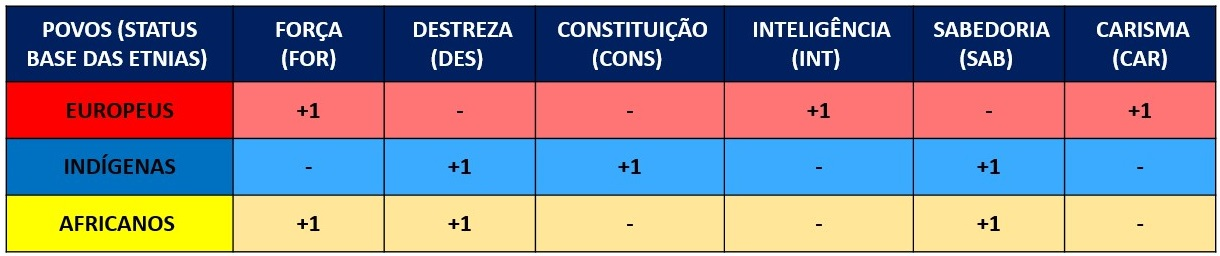
\includegraphics[width = 1.3 \CaptionWidth]{tbCriacaoPesonagem}
\SourceOrNote{Autoria Própria (2024)}
\\
\end{table}
\\
\end{itemize}

\\
\begin{table}[!h]
\centering
\SetCaptionWidth{\ifbool{@LayoutA}{0.7}{0.72}\linewidth}
\caption{Profissões}%
\label{grph:Prof}
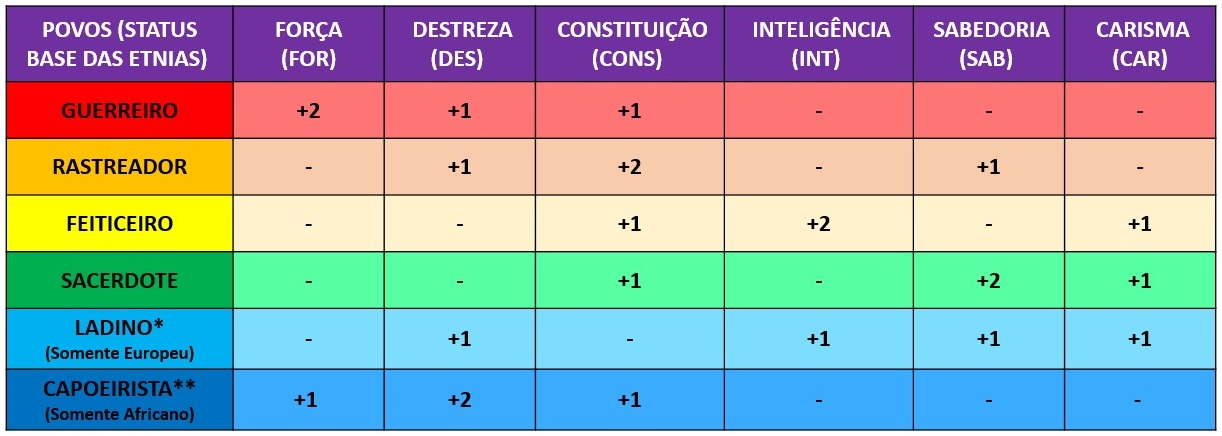
\includegraphics[width = 1.3 \CaptionWidth]{tbProfissoes}
\SourceOrNote{Autoria Própria (2024)}
\\
\end{table}
\\

As bonificações raciais concedidas pelas etnias escolhidas são aplicadas ao perfil do estudante. Após essa escolha, os estudantes poderão selecionar suas profissões, que receberão bônus específicos em seus status. A análise combinatória resulta em um total de 12 possibilidades de criação de personagens, cada um começando com 7 pontos de criação iniciais. Em seguida, o sistema concederá mais 6 pontos de bonificação, que poderão ser distribuídos conforme os estudantes desejarem, desde que nenhum atributo fique zerado ou maior que 4 no início da campanha. Durante o jogo, os estudantes terão a oportunidade de ganhar mais pontos de atributos e distribuí-los entre seus status de acordo com a orientação e o progresso no jogo. 
\\

\\
\begin{itemize}
\\
  \item \textbf{Iniciando a Campanha:} Dependendo da etnia escolhida, o sistema dará início à Campanha em uma localidade específica. Como ponto de partida, serão oferecidos escolhas e desafios aos estudantes, permitindo que escolham o caminho e percurso a seguir. O nível de dificuldade desses desafios será determinado pela análise do sistema, com base no banco de dados do Google Classroom vinculado durante o cadastro do estudante. Este banco de dados fornece um pré-diagnóstico do nível de desenvolvimento do estudante, com base na Matriz de Referência para o teste de Língua Portuguesa do SAEB para a 3ª Série do Ensino Médio (que é a mesma para o 9º Ano do Ensino Fundamental dos Anos Finais). Essa matriz é composta por seis tópicos relacionados às habilidades desenvolvidas pelos estudantes, cada um com um conjunto de descritores ligados às competências desenvolvidas. 
\\
 \item \textbf{Escolhas de Desafios:} As escolhas de desafios serão baseadas na Escala de Proficiência em Língua Portuguesa, utilizando as descrições de níveis correspondentes. Esta escala de proficiência é composta por níveis progressivos e cumulativos, o que significa que ela está organizada em níveis que vão do menor para o maior, e cada nível de desempenho acumula os conhecimentos e habilidades dos níveis anteriores. Portanto, quando um grupo de estudantes é posicionado em um determinado nível da escala, presume-se que esses estudantes tenham desenvolvido não apenas as habilidades descritas nesse nível, mas também as habilidades dos níveis anteriores. 
\\
\item \textbf{Conquitas e Evolução:} Os estudantes terão acesso a uma tela que mostrará a progressão de seus personagens, exibindo as conquistas adquiridas ao longo da jornada. Isso incluirá o avanço de nível do personagem, ganho de Pontos de Experiência (PE), obtenção de itens e benefícios após a conclusão dos desafios, bem como a capacidade de desbloquear Tokens para melhorar seus personagens. Esses dados serão transferidos para a visão do professor, permitindo que acompanhe a evolução dos estudantes e realize uma análise diagnóstica das defasagens sanadas e das dificuldades ainda presentes. Isso possibilitará o desenvolvimento e aplicação de planos de ação para realinhar a aprendizagem dos estudantes, consolidando os conhecimentos adquiridos e aprofundando aqueles que já possuíam. 
\\
\item \textbf{Período e Desenvolvimento:} Esta proposta é anual e organiza as Trilhas Pedagógicas Gamificadas em "Temporadas" distintas, cada uma composta por 4 Capítulos. O objetivo é desenvolver as habilidades, competências e conteúdos do respectivo currículo em questão, organizados por Escala de Proficiência, Level Cap (limite máximo de nível que o jogador pode alcançar durante um determinado período) e EPIC LEVEL (todos os pontos adicionais que o estudante conseguir durante o Level Cap serão convertidos ao término da Temporada em Níveis Épicos, concedendo benefícios adicionais aos jogadores).
\\
\end{itemize}

Ao fazer login no sistema, os professores terão acesso aos seguintes menus:
\\

\\
\begin{itemize}
\\
\item \textbf{Cadastro da Turma no Sistema:} O professor tem suas aulas atribuídas, e essa informação é vinculada ao seu perfil institucional na Secretaria Escolar Digital. Como o email do professor é da Google, ele tem acesso aos dados das turmas disponíveis para acompanhamento no Google Classroom. Com o email institucional, o professor se cadastra no sistema do TPG System. Isso permite o compartilhamento de informações das turmas entre os dois sistemas, garantindo a integração dos dados e facilitando o acompanhamento das atividades e evolução dos estudantes pelo professor.
\\

\item \textbf{Iniciando a Campanha e Escolhendo os Desafios:} Com base nos dados da turma, o professor seleciona o conjunto de habilidades e competências que serão trabalhados ao longo do bimestre. Ele também indica a quantidade de desafios desejados e seus níveis de dificuldade para a sala, utilizando as informações da Escala de Proficiência do SAEB. Essa escala é agrupada no SARESP em quatro níveis de proficiência (Abaixo do Básico, Básico, Adequado e Avançado), os quais são definidos a partir das expectativas de aprendizagem (conteúdos, competências e habilidades) estabelecidos para cada ano/série e disciplina no currículo do Estado de São Paulo (\Cref{grph:tabNivelProf}).
\\

\begin{table}[!h]
\centering
\SetCaptionWidth{\ifbool{@LayoutA}{0.7}{0.72}\linewidth}
\caption{Níveis de Proficiências}%
\label{grph:tabNivelProf}
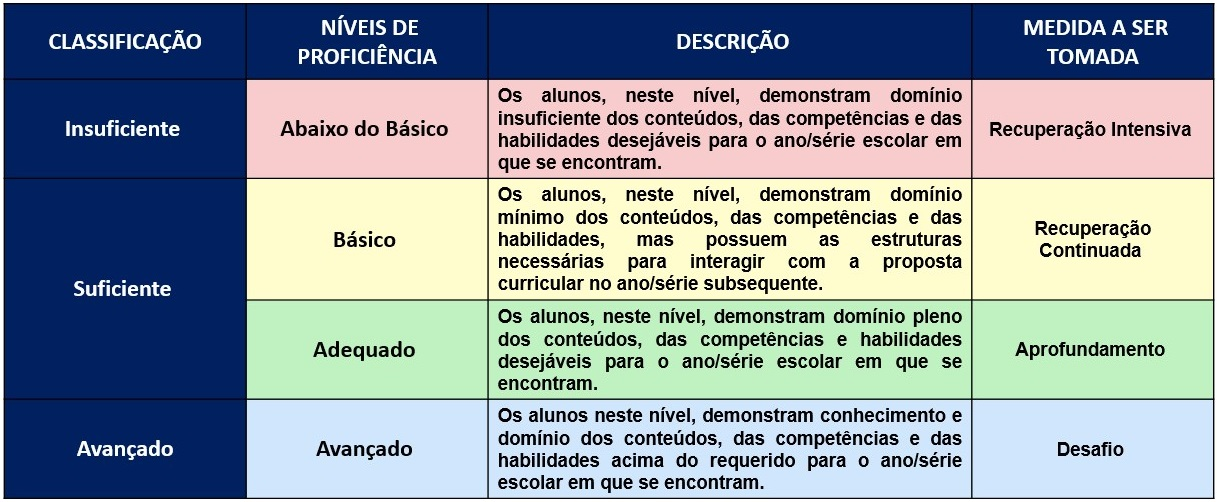
\includegraphics[width = 1.3 \CaptionWidth]{Illustrations/tbNivelProficencia.jpg}
\SourceOrNote{Elaboração própria a partir do Boletim SARESP (2022).}
\\
\end{table}
\\

\item \textbf{Conquitas e Evolução:} Através do seu perfil no TPG System, o professor terá acesso aos relatórios de evolução e conquistas dos estudantes. Ele poderá visualizar as alternativas escolhidas por eles para responder a um desafio, o tempo que levaram para concluir a atividade, bem como seus acertos e erros. Todas essas informações são cruciais para realizar o balanceamento dos resultados e autorizar as progressões e conquistas obtidas pelos estudantes. Dessa forma, o professor terá duas visões do processo evolutivo: uma dentro do jogo e outra no desenvolvimento no mundo real.
\\

\item \textbf{Período e Desenvolvimento:} Os professores, com base nos relatórios de aprendizagem disponibilizados pelo TPG System, poderão articular a aprendizagem adquirida no jogo para ser testada e validada no ambiente real, por meio de situações de aprendizagem convencionais. Isso permite que essa metodologia valide aquilo que foi desenvolvido de forma lúdica e gamificada, possibilitando que os estudantes ressignifiquem seus conhecimentos e percebam que a aprendizagem pode ser verdadeiramente impactante e transformadora. A contextualização dessas práticas com a vivência no cotidiano torna a aprendizagem integral.
\\
\end{itemize}

\section*{ESTADO DA ARTE} \label{sect:estadoarte}

Este artigo busca traçar a evolução da gamificação na educação, desde suas raízes iniciais até seu estado atual, e examinar como essa abordagem pode ser efetivamente implementada para promover a aprendizagem e o engajamento dos estudantes na era digital. Ao refletir sobre o passado, podemos informar e inspirar as práticas futuras na integração bem-sucedida de jogos e educação.
\\

Os primeiros levantamentos sobre a utilização da metodologia de gamificação na educação remonta ao final dos anos 1990 e início dos anos 2000, liderado por Thomas W. Malone, do MIT, em colaboração com seus colegas. Em \citep{malone2021fazendo}, publicaram o influente artigo "Tornando a aprendizagem divertida: uma taxonomia de motivações intrínsecas para a aprendizagem", no qual discutiram a importância de motivar os estudantes de forma intrínseca para a aprendizagem, propondo uma taxonomia de motivações essenciais. Embora não seja explicitamente um estudo sobre gamificação na educação contemporânea, esse trabalho é frequentemente citado como uma das primeiras explorações acadêmicas da conexão entre motivação intrínseca e aprendizagem, aspectos cruciais para o desenvolvimento da gamificação educacional.
\\

De acordo com o artigo: " Dos elementos de design de jogos à ludicidade: definindo "gamificação", \citep{deterding2011game}, fornecem uma definição fundamental para o termo “gamificação”, explorando a transição dos elementos de design de jogos para o conceito mais amplo de “gamefulness”, abordando como os elementos de design presentes nos jogos podem ser aplicados em contextos não relacionados a jogos, como educação, saúde, marketing e ambiente de trabalho, para promover o engajamento e motivar o comportamento desejado.
\\

Já em "Um guia prático para a gamificação na educação", \citep{hsin2013practitioner}, apresenta um guia prático destinado a educadores interessados em implementar a gamificação em suas práticas de ensino. Este guia oferece insights valiosos sobre como usar a gamificação de forma eficaz na educação, fornecendo orientações e estratégias específicas para projetar e implementar experiências de aprendizado gamificadas. Ele visa ajudar os educadores a entender os princípios fundamentais da gamificação e como aplicá-los de maneira significativa em ambientes educacionais. 
\\

Em o estudo, “A gamificação funciona? - uma revisão da literatura de estudos empíricos sobre gamificação” \citep{hamari2014does}, revisa uma série de pesquisas empíricas sobre gamificação e seu impacto em diversas áreas, incluindo educação. Ao examinar o corpo de literatura existente, os autores investigam se a gamificação é eficaz em alcançar seus objetivos propostos, abordando questões como elementos de gamificação mais eficazes, contextos de sucesso e desafios enfrentados na implementação dessas estratégias.
\\

O artigo "Um teste empírico da teoria da aprendizagem gamificada: O efeito das tabelas de classificação no tempo gasto na tarefa e no desempenho acadêmico",  \citep{landers2014empirical} é um estudo empírico que investiga o impacto dos placares de líderes na motivação e desempenho dos estudantes. Especificamente, os autores examinam como a presença de placares de líderes, uma característica comum em ambientes gamificados, influencia o tempo dedicado à tarefa pelos estudantes e seu desempenho acadêmico.
\\

Em "Gamificação em teoria e ação: Uma pesquisa" \citep{seaborn2015gamification},  retoma a análise abrangente sobre a teoria e prática da gamificação. Reforça como a gamificação é aplicada em uma variedade de contextos, examinando tanto os fundamentos teóricos por trás dessa abordagem quanto exemplos práticos de sua implementação. O estudo aborda questões como motivação, engajamento do usuário e design de sistemas gamificados, além de discutir os efeitos da gamificação em diferentes áreas, incluindo educação, negócios e saúde.
\\

A correlação entre o uso da gamificação na educação e os índices de melhoria na qualidade educacional de um país é um tema complexo e multifacetado. Embora existam estudos e evidências que sugerem benefícios no engajamento dos estudantes e no desempenho acadêmico decorrentes da gamificação, é difícil atribuir diretamente essa prática a melhorias específicas nos índices educacionais de um país.  
\\

Alguns exemplos de países que têm explorado ativamente a gamificação na educação incluem os Estados Unidos, Finlândia, Singapura, Austrália, Reino Unido, Coreia do Sul e Canadá. Esses países frequentemente estão na vanguarda da inovação educacional e têm sistemas educacionais que incentivam a experimentação e o desenvolvimento de novas práticas pedagógicas com o uso de metodologias ativas de aprendizagem, e tendem a compartilhar algumas características comuns, como: 
\\

\begin{enumerate}
    \item \textbf{Investimento em Tecnologia Educacional:} Nações que investem significativamente em tecnologia educacional têm mais probabilidade de integrar a gamificação de forma eficaz. Isso inclui não apenas o acesso a dispositivos e infraestrutura tecnológica nas escolas, mas também o desenvolvimento de plataformas e aplicativos educacionais que incorporam elementos de gamificação;
\\
    \item \textbf{Políticas Educacionais Progressistas:} Países com políticas educacionais progressistas e flexíveis estão mais abertos a experimentar novas abordagens pedagógicas, incluindo a gamificação. Flexibilidade curricular e autonomia escolar podem permitir que as escolas implementem práticas inovadoras de ensino;
\\
    \item \textbf{Formação de Professores:} A formação adequada de professores é essencial para a implementação eficaz da gamificação na sala de aula. Países que investem em programas de desenvolvimento profissional para capacitar os educadores a integrar a gamificação em seu ensino estão mais bem posicionados para alcançar sucesso nessa área;
\\
    \item \textbf{Cultura de Inovação Educacional:} Nações com uma cultura de inovação educacional e uma mentalidade aberta à experimentação tendem a adotar mais prontamente abordagens como a gamificação. Isso pode ser incentivado por meio de políticas que apoiam a pesquisa e o desenvolvimento de novas práticas educacionais;  
\\
    \item \textbf{Engajamento dos Estudantes:} Países que priorizam o engajamento dos estudantes e reconhecem a importância do aspecto motivacional no processo de aprendizagem são mais propensos a adotar a gamificação como uma estratégia para tornar a educação mais envolvente e relevante para os estudantes.
\\
\end{enumerate}

Segundo o estudo intitulado: "Game Design: Plataforma Gamificada como Inovação Tecnológica na Educação" \cite{de2022game}, investigou o uso de plataformas gamificadas na educação online, especialmente no ensino básico, e mapeou os mecanismos de jogos mais utilizados. O estudo, caracterizado como exploratório, utilizou uma revisão da literatura para compreender o uso da gamificação na educação e uma análise de similares. Os resultados destacam a gamificação como uma tendência emergente na educação, identificando lacunas de pesquisa, como a necessidade de aplicação dos elementos de interação na educação, estudos de experiência do usuário e pesquisas a longo prazo. Este estudo pode beneficiar educadores em busca de plataformas gamificadas e profissionais envolvidos no desenvolvimento e aprimoramento dessas ferramentas.  
\\

Atualmente, algumas plataformas pedagógicas incorporam recursos de gamificação e elementos de Role Playing Game (RPG), mas nem todas conseguem integrar plenamente essas duas essências. Muitas delas negligenciam aspectos fundamentais do RPG, como a estruturação de personagens, a distribuição de Pontos de Atributos e Pontos de Habilidades. Esses elementos são cruciais para permitir que os jogadores personalizem e adaptem seus personagens de acordo com suas preferências e estratégias de jogo. Além disso, é observado que essas plataformas gamificadas geralmente não utilizam o recurso de "Quest" (missão ou tarefa), que é uma atividade ou objetivo atribuído aos personagens pelos narradores do jogo, pelo sistema do jogo ou por outros personagens não jogadores (NPCs). As quests desempenham um papel fundamental na narrativa e na jogabilidade de muitos RPGs, proporcionando aos jogadores objetivos específicos para superar desafios e conquitar recompensas.
\\

Com base nessas observações, três plataformas se destacam por fazer uso desses recursos:
\\

\\
\begin{enumerate}
    \item \textbf{Quest Atlantis:} Plataforma educacional baseada em jogos desenvolvida pela University of Indiana, nos Estados Unidos. Criada por Sasha Barab, Chris Dede e Kurt Squire, com contribuições de muitos outros pesquisadores e desenvolvedores, o projeto começou no final da década de 1990 e continuou a se desenvolver ao longo dos anos seguintes. O "Quest Atlantis" é um ambiente virtual de aprendizagem projetado para envolver os estudantes em experiências educacionais imersivas e interativas, permitindo que eles explorem diferentes temas e realizem missões enquanto aprendem conceitos acadêmicos;  
\\ 
\item \textbf{3DGameLab:} Plataforma de aprendizagem baseada em jogos que permite aos educadores criar cursos e atividades gamificadas para seus estudantes. Desenvolvido por Lisa Dawley e Chris Haskell na Boise State University, nos Estados Unidos, o projeto começou em 2011. Dawley e Haskell fundaram o "3D Game Lab" como um ambiente de aprendizagem inovador e envolvente para apoiar a educação baseada em jogos. A plataforma foi projetada para integrar elementos de jogos e gamificação no processo de ensino e aprendizagem, proporcionando uma experiência mais motivadora para os estudantes;
\\
\item \textbf{CassCraft:} Plataforma de gamificação para salas de aula desenvolvida por Shawn Young. O projeto começou em 2013, quando Young, um professor de física no Canadá, criou o "Classcraft" como uma maneira de tornar o aprendizado mais envolvente e motivador para seus estudantes. Desde então, a plataforma cresceu e se tornou uma ferramenta popular usada por educadores em todo o mundo para gamificar o ambiente de sala de aula e promover o engajamento dos estudantes. 
\\
\end{enumerate}

Com base na investigação conduzida sobre o tema proposto, "Trilha Pedagógica Gamificada com Elementos de RPG: Uma Abordagem para a Educação", e comparando-a com estudos anteriores realizados por outras linhas de pesquisa, observa-se que é viável desenvolver uma aplicação capaz de envolver tanto os educadores quanto os estudantes. Essa aplicação visa renovar práticas pedagógicas por meio do uso de metodologias ativas, que podem ser implementadas tanto de forma online quanto offline, de maneira síncrona ou assíncrona. 
\\

A proposta busca correlacionar o aprendizado dos estudantes, fornecendo dados e relatórios detalhados de seu desenvolvimento e progresso. Esses relatórios são apresentados por meio de gráficos e índices, permitindo que os professores compreendam o percurso de cada estudante e identifiquem suas necessidades específicas de intervenção, recuperação, consolidação ou aprofundamento de conhecimentos. Essa abordagem visa atender às demandas individuais de todos os estudantes envolvidos na ação educacional. 
\\






\section*{METODOLOGIA} \label{sect:metodologia}

As metodologias aqui elencadas visam contribuir para especificar de forma prática as etapas do desenvolvimento do Sistema de Trilha Pedagógica Gamificada com Elementos de RPG. Espera-se que sejam aplicadas de forma prática nos mais diversos contextos pedagógicos e educacionais, armazenando e apresentando dados de forma acessível e informativa, facilitando o monitoramento e a tomada de decisões pelas equipes docentes envolvidas na aplicação e desenvolvimento desta ação, junto aos seus estudantes.
\\

\textbf{Desenvolvimento de Protótipos de Interface:} O Figma, uma plataforma de colaboração para design de interfaces e protótipos, será utilizada como ambiente colaborativo para desenvolver os protótipos da interface de usuário da aplicação. Isso permitirá que a equipe de design trabalhe de forma conjunta, compartilhando conceitos e recebendo feedback em tempo real, garantindo uma interface intuitiva e esteticamente atrativa para o Sistema de Trilha Pedagógica Gamificada com Elementos de RPG.
\\

\textbf{Planejamento do Modelo de Negócios:} O Business Model Canvas, uma ferramenta estratégica, será empregado no planejamento e esboço do modelo de negócios específico para o sistema de identificação e diagnóstico. Será utilizado para criar um modelo visual que descreva como o projeto se encaixa no contexto do monitoramento do avanço pedagógico dos estudantes. A equipe usará o Canvas para identificar parceiros estratégicos, recursos essenciais, atividades fundamentais e fontes de receita, mantendo a coesão com os objetivos do sistema.
\\

\textbf{Modelagem do Sistema de Software:} A UML (Unified Modeling Language) será aplicada como linguagem visual na modelagem do sistema de software. A plataforma utilizada para essa etapa sera o Lucidchart. Através de um estudo de caso, a UML será usada para representar elementos cruciais do sistema, como a interface de usuário, o fluxo de informações e as interações entre os módulos do sistema de identificação e diagnóstico do avanço pedagógico dos estudantes, contribuindo para uma compreensão completa e documentação eficaz da arquitetura do sistema.
\\

\textbf{Modelagem do Banco de Dados:} O DER (Diagrama de Entidade e Relacionamento) será adotado para modelar a estrutura do banco de dados do sistema, definindo entidades relevantes, como o público-alvo que utilizará o sistema (estudantes e professores), escala de proficiência, nível de proficiência do estudante, evolução de aprendizagem, habilidades a serem desenvolvidas, consolidadas ou aprofundadas, e nível de avanço do estudante e da sala de aula como um todo.
\\

\textbf{Estruturação do Banco de Dados:} Para a estruturação do banco de dados da aplicação, será utilizado o programa XAMPP, que possui um pacote com os principais servidores de código aberto, simulando o funcionamento pleno de consultas e conexões entre o sistema criado e o banco de dados, com suporte às linguagens PHP e Perl. Para a criação do banco de dados, optou-se pelo MySQL, por ser um sistema de banco de dados que utiliza a Linguagem de Consulta Estruturada (SQL - Structured Query Language), sendo de fácil utilização e integração com diferentes linguagens de programação.
\\

\textbf{Desenvolvimento do Sistema:} A equipe de desenvolvimento optou pelo editor de código-fonte Visual Studio Code, por possuir suporte de depuração, controle de versionamento Git incorporado, entre outros recursos que facilitam a codificação em Node.js, permitindo rodar códigos JavaScript fora dos navegadores. Este editor facilita a estruturação da aplicação, tanto no front-end quanto no back-end, em um único local. Nesta etapa, o foco do desenvolvimento será a versão desktop.
\\

\textbf{Criação dos Personagens:} Para a criação dos personagens, foi utilizada a plataforma Hero Forge, que permite projetar figuras de forma customizável, usando tecnologia de impressão 3D e na web. Isso permite visualizar as figuras em 3D e exportar imagens para a aplicação.
\\

\section*{RESULTADOS PRELIMINARES}\label{sect:resultados}

Os resultados obtidos abrangem várias etapas importantes do projeto, até o presente momento. Inicialmente, incluem a prototipagem das telas da aplicação móvel, que posteriormente será traduzida e compilada utilizando uma linguagem de programação adequada para ser implementada no Sistema em Node.js, destinado ao uso em desktop. Além disso, são apresentados os estudos realizados para o Business Model Canvas, bem como a modelagem do banco de dados, tanto no nível conceitual quanto lógico. Essa modelagem inclui os Diagramas de Classe e de Objetos, os quais estão segmentados pelos perfis do Professor e do Estudante, detalhando as correlações das entidades com seus atributos específicos.
\\

Adicionalmente, são elaboradas as estruturas sistêmicas na forma do Diagrama de Caso de Uso (DCU), os quais são diferenciados de acordo com os perfis do Professor e do Estudante. Estes diagramas destacam as permissões e acessos individuais de cada usuário no sistema. Por fim, é apresentado o Diagrama de Rede, ilustrando a maneira pela qual os usuários acessam e transmitem dados dentro da aplicação.
\\

Além das etapas mencionadas, são realizados cálculos para verificar a eficácia do algoritmo de ordenação implementado no sistema. Esses cálculos são cruciais para avaliar o desempenho e a eficiência do algoritmo em diferentes cenários.
\\

\begin{itemize}

\item \textbf{Business Model Canvas}
\\

\end{itemize}

O desenvolvimento de um modelo de negócios demanda uma atenção primordial na satisfação das necessidades e expectativas do cliente. Para viabilizar o Sistema de Trilha Pedagógica Gamificada, é essencial conduzir estudos e investir no âmbito da tecnologia educacional e das metodologias direcionadas ao desenvolvimento curricular, seja em formato digital, conectado ou offline. Além disso, é imperativo estabelecer parcerias estratégicas com redes de ensino, setor privado e empresas especializadas no desenvolvimento de ferramentas educacionais, as quais contribuirão para a concretização dos objetivos delineados no Business Model Canvas (\Cref{fig:imgBMC.jpg}).
\\

\begin{figure}[!h]
\centering
\caption{BUSINESS MODEL CANVAS - TPG System}%
\label{fig:imgBMC.jpg}
\includegraphics[scale=0.3]{Illustrations/imgBMC.jpg}
\SourceOrNote{Autoria Própria (2024)}
\end{figure}
\pagebreak

\begin{itemize}

\item \textbf{Prototipação do Sistema Mobile - Figma:}
\\

\end{itemize}

A (\Cref{fig:Tela1}) mostra a tela inicial do TPG System, acessada pelo dispositivo móvel. Este sistema permite que o usuário realize seu cadastro (\Cref{fig:Tela2}), caso seja a primeira vez que estiver acessando, ou faça login (\Cref{fig:Tela3}), escolhendo seu perfil de Professor ou Estudante para prosseguir.
\\

\begin{figure}[!h]
\centering
\caption{Tela de Apresentação do Sistema - TPG System}%
\label{fig:Tela1}
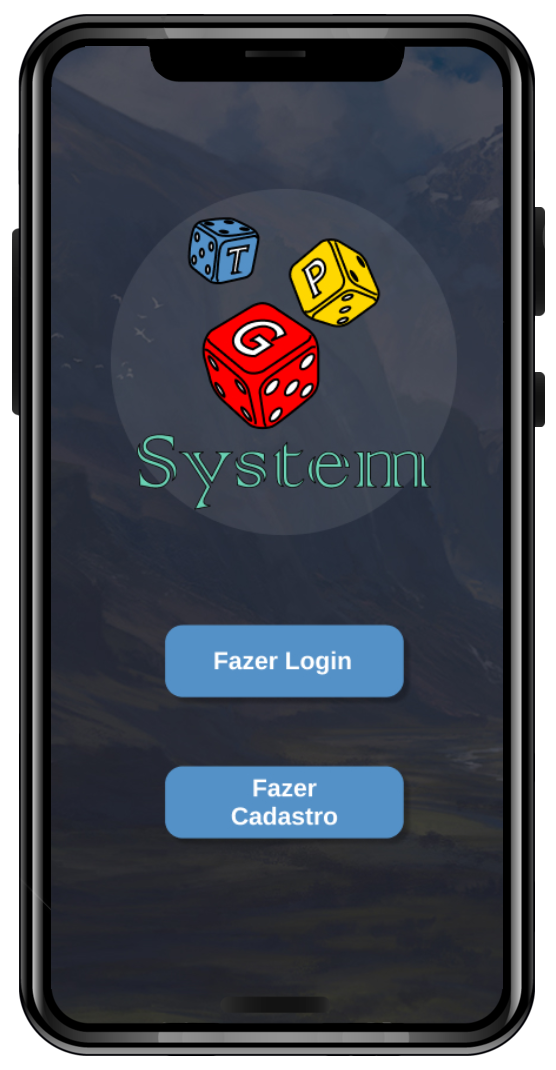
\includegraphics[scale=0.20]{Illustrations/Tela1.png}
\SourceOrNote{Autoria Própria (2024)}
\end{figure}

\begin{figure}[!h]
\centering
\caption{Tela de Cadastro - TPG System}%
\label{fig:Tela2}
\includegraphics[scale=0.20]{Illustrations/Tela2.png}
\SourceOrNote{Autoria Própria (2024)}
\end{figure}

\begin{figure}[!h]
\centering
\caption{Tela de Login - TPG System}%
\label{fig:Tela3}
\includegraphics[scale=0.20]{Illustrations/Tela3.png}
\SourceOrNote{Autoria Própria (2024)}
\end{figure}
\\

No perfil de Professor, é liberado o acesso para a realização do “Cadastro da Aventura” (\Cref{fig:Tela4}), que oferece as seguintes opções de menu (\Cref{fig:Tela5}):
\\
\pagebreak

\begin{figure}[!h]
\centering
\caption{Perfil do Professor - Realização de Cadastro - TPG System}%
\label{fig:Tela4}
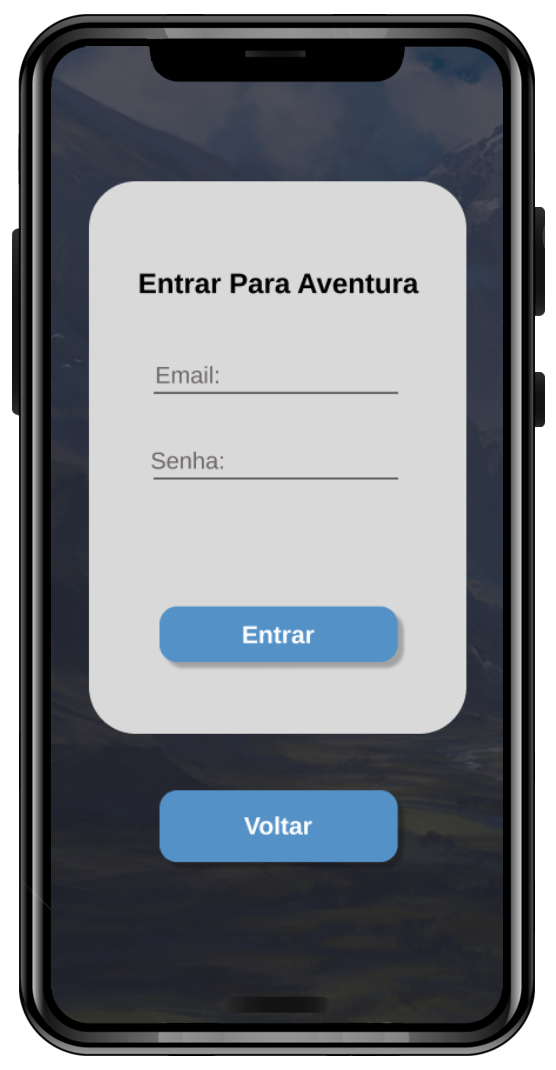
\includegraphics[scale=0.20]{Illustrations/Tela4.png}
\SourceOrNote{Autoria Própria (2024)}
\end{figure}

\begin{figure}[!h]
\centering
\caption{Perfil do Professor - Menu de Consultas e Opções - TPG System}%
\label{fig:Tela5}
\includegraphics[scale=0.20]{Illustrations/Tela5.png}
\SourceOrNote{Autoria Própria (2024)}
\end{figure}

“Iniciar”, onde o professor pode acompanhar o desenvolvimento dos usuários com o sistema, que reconhece as interações do usuário com os desafios, funcionando como um teste prático. Isso permite que o professor ajuste manualmente os níveis de dificuldade e as habilidades relacionadas;
\\

“Opções”, que abre uma nova tela (\Cref{fig:Tela6}), permitindo a consulta dos relatórios sistêmicos via desenvolvimento dos estudantes, na opção “Verificar Estudante”, disponível após a realização dos cadastros sistêmicos das turmas lecionadas, ou a criação de uma Nova Turma (\Cref{fig:Tela7});
\\

\begin{figure}[!h]
\centering
\caption{Perfil do Professor - Opções de Consulta de Relatórios ou Cadastro de Turmas - TPG System}%
\label{fig:Tela6}
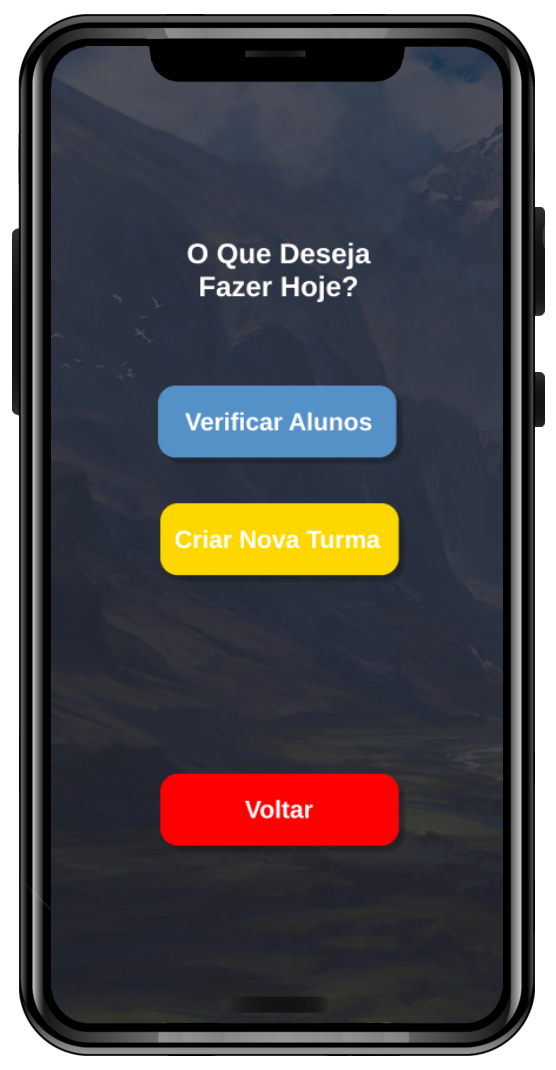
\includegraphics[scale=0.20]{Illustrations/Tela6.png}
\SourceOrNote{Autoria Própria (2024)}
\end{figure}

\begin{figure}[!h]
\centering
\caption{Perfil do Professor - Cadastro da Turma no sistema - TPG System}%
\label{fig:Tela7}
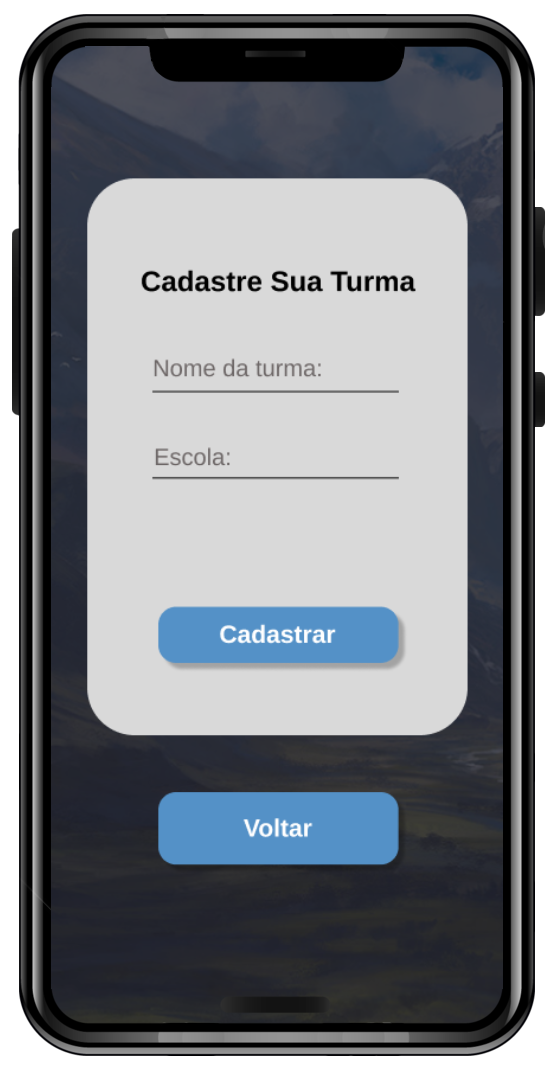
\includegraphics[scale=0.20]{Illustrations/Tela7.png}
\SourceOrNote{Autoria Própria (2024)}
\end{figure}

“Sair”, que realiza o logout do sistema.
\\
\pagebreak

No perfil de Estudante, é necessário realizar o “Cadastro de Aventureiro” (\Cref{fig:Tela8}) para liberar o acesso à criação de personagens (atualmente, o sistema oferece personagens prontos para uso e familiarização). Após o cadastro, o estudante pode explorar o sistema (\Cref{fig:Tela9}) e, ao logar-se, é direcionado para uma nova tela (\Cref{fig:Tela10}) com os seguintes menus:
\\

\begin{figure}[!h]
\centering
\caption{Perfil do Estudante - Cadastro de Aventureiro - TPG System}%
\label{fig:Tela8}
\includegraphics[scale=0.20]{Illustrations/Tela8.png}
\SourceOrNote{Autoria Própria (2024)}
\end{figure}

\begin{figure}[!h]
\centering
\caption{Perfil do Estudante - Acesso ao Sistema Pedagógico Gamificado - TPG System}%
\label{fig:Tela9}
\includegraphics[scale=0.20]{Illustrations/Tela9.png}
\SourceOrNote{Autoria Própria (2024)}
\end{figure}

\begin{figure}[!h]
\centering
\caption{Perfil do Estudante - Menus e Opções - TPG System}%
\label{fig:Tela10}
\includegraphics[scale=0.20]{Illustrations/Tela10.png}
\SourceOrNote{Autoria Própria (2024)}
\end{figure}

“Iniciar”, onde o estudante inicia a Trilha Pedagógica Gamificada, sendo direcionado ao ponto de partida no mapa relacionado ao personagem escolhido;
\\

“Opções”, onde o estudante pode verificar sua evolução no jogo, as conquistas obtidas e as derrotas nos desafios, apresentados em um relatório personalizado;
\\

“Sair”, que realiza o logout do sistema.
\\

Na tela “Qual Tema da sua Aventura?” (\Cref{fig:Tela11}), o estudante pode escolher trilhas específicas de acordo com seus interesses ou necessidades de desenvolvimento de habilidades e competências. Após selecionar o componente desejado, aparece um sub-menu com as aventuras disponíveis (\Cref{fig:Tela12}).
\\

\begin{figure}[!h]
\centering
\caption{Perfil do Estudante - Escolha de Temas (Componentes) - TPG System}%
\label{fig:Tela11}
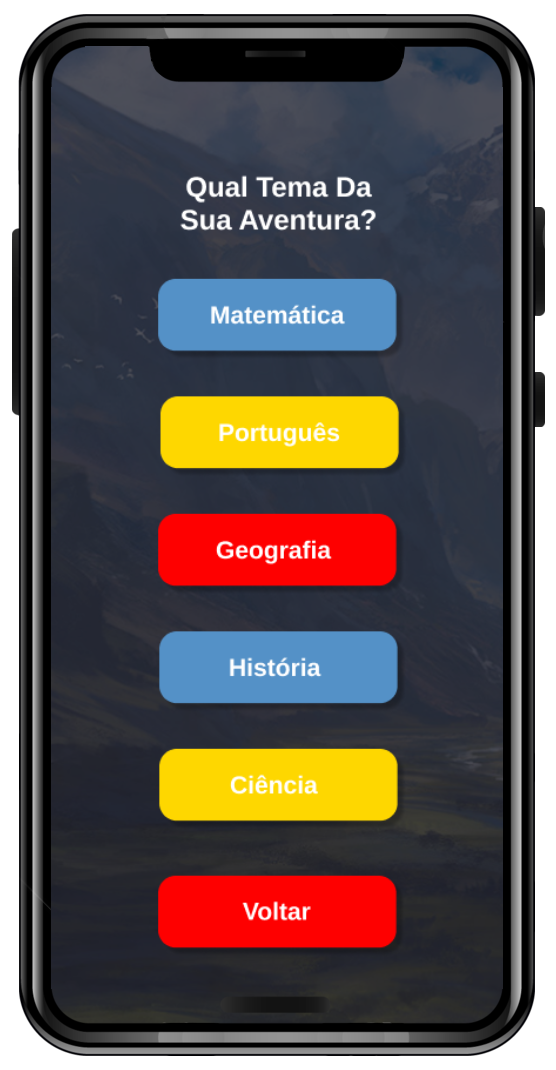
\includegraphics[scale=0.20]{Illustrations/Tela11.png}
\SourceOrNote{Autoria Própria (2024)}
\end{figure}

\begin{figure}[!h]
\centering
\caption{Perfil do Estudante - Escolha da Aventura dentro do Tema - TPG System}%
\label{fig:Tela12}
\includegraphics[scale=0.20]{Illustrations/Tela12.png}
\SourceOrNote{Autoria Própria (2024)}
\end{figure}

Ao iniciar o jogo, o estudante vê um mapa (\Cref{fig:Tela13}) com pontos de interesse que direcionam para desafios intelectuais ou de combate. Neste menu (\Cref{fig:Tela14}), o estudante pode consultar os dados de seu Personagem (\Cref{fig:Tela15}), bem como seu Inventário e as Informações de sua Conta, além de ter a opção de sair do sistema.
\\

\begin{figure}[!h]
\centering
\caption{Perfil do Estudante - Mapa da Aventura - TPG System}%
\label{fig:Tela13}
\includegraphics[scale=0.20]{Illustrations/Tela13.png}
\SourceOrNote{Autoria Própria (2024)}
\end{figure}

\begin{figure}[!h]
\centering
\caption{Perfil do Estudante - Menu - TPG System}%
\label{fig:Tela14}
\includegraphics[scale=0.20]{Illustrations/Tela14.png}
\SourceOrNote{Autoria Própria (2024)}
\end{figure}

\begin{figure}[!h]
\centering
\caption{Perfil do Estudante - Status do Personagem - TPG System}%
\label{fig:Tela15}
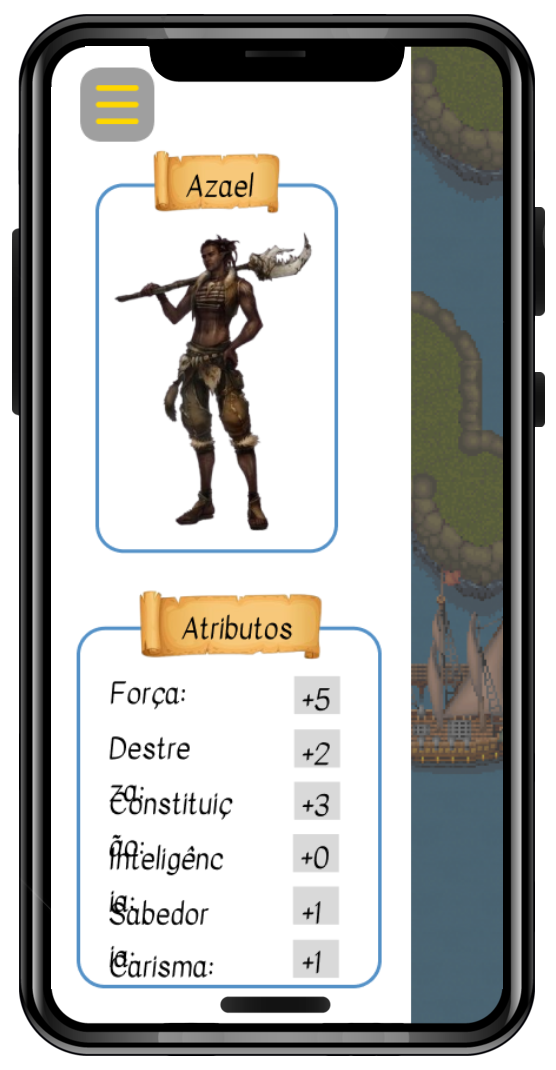
\includegraphics[scale=0.20]{Illustrations/Tela15.png}
\SourceOrNote{Autoria Própria (2024)}
\end{figure}
\\
\pagebreak
Está sendo estudada a possibilidade de que, ao sair, as informações de evolução não sejam perdidas, permitindo que, ao relogar no sistema, o estudante continue de onde parou. Este recurso possibilita uma continuidade na aprendizagem de forma dinâmica, sem a necessidade de reiniciar a etapa do zero.
\\
\pagebreak

\begin{itemize}

\item \textbf{Modelagem Banco de Dados - Conceitual e Lógico:}
\\

\end{itemize}

Na Modelagem Conceitual (\Cref{fcht:imgdgMC.jpg}), a ênfase foi dada à representação das associações entre as entidades, destacando seus atributos e, principalmente, os acessos através de chaves estrangeiras. Essa abordagem tem o objetivo de orientar a equipe de desenvolvimento na estruturação do sistema de forma a facilitar atualizações e modificações, permitindo a implementação rápida e precisa de novas funcionalidades. Esse estudo é solidificado por meio do diagrama da Modelagem Lógica (\Cref{fcht:imgdgML.jpg}), o qual representa de maneira mais concreta e detalhada as estruturas de dados e os relacionamentos definidos na etapa conceitual.
\\

\begin{flowchart}[!h]
\centering
\caption{Diagrama de Modelagem Conceitual - TPG System}%
\label{fcht:imgdgMC.jpg}
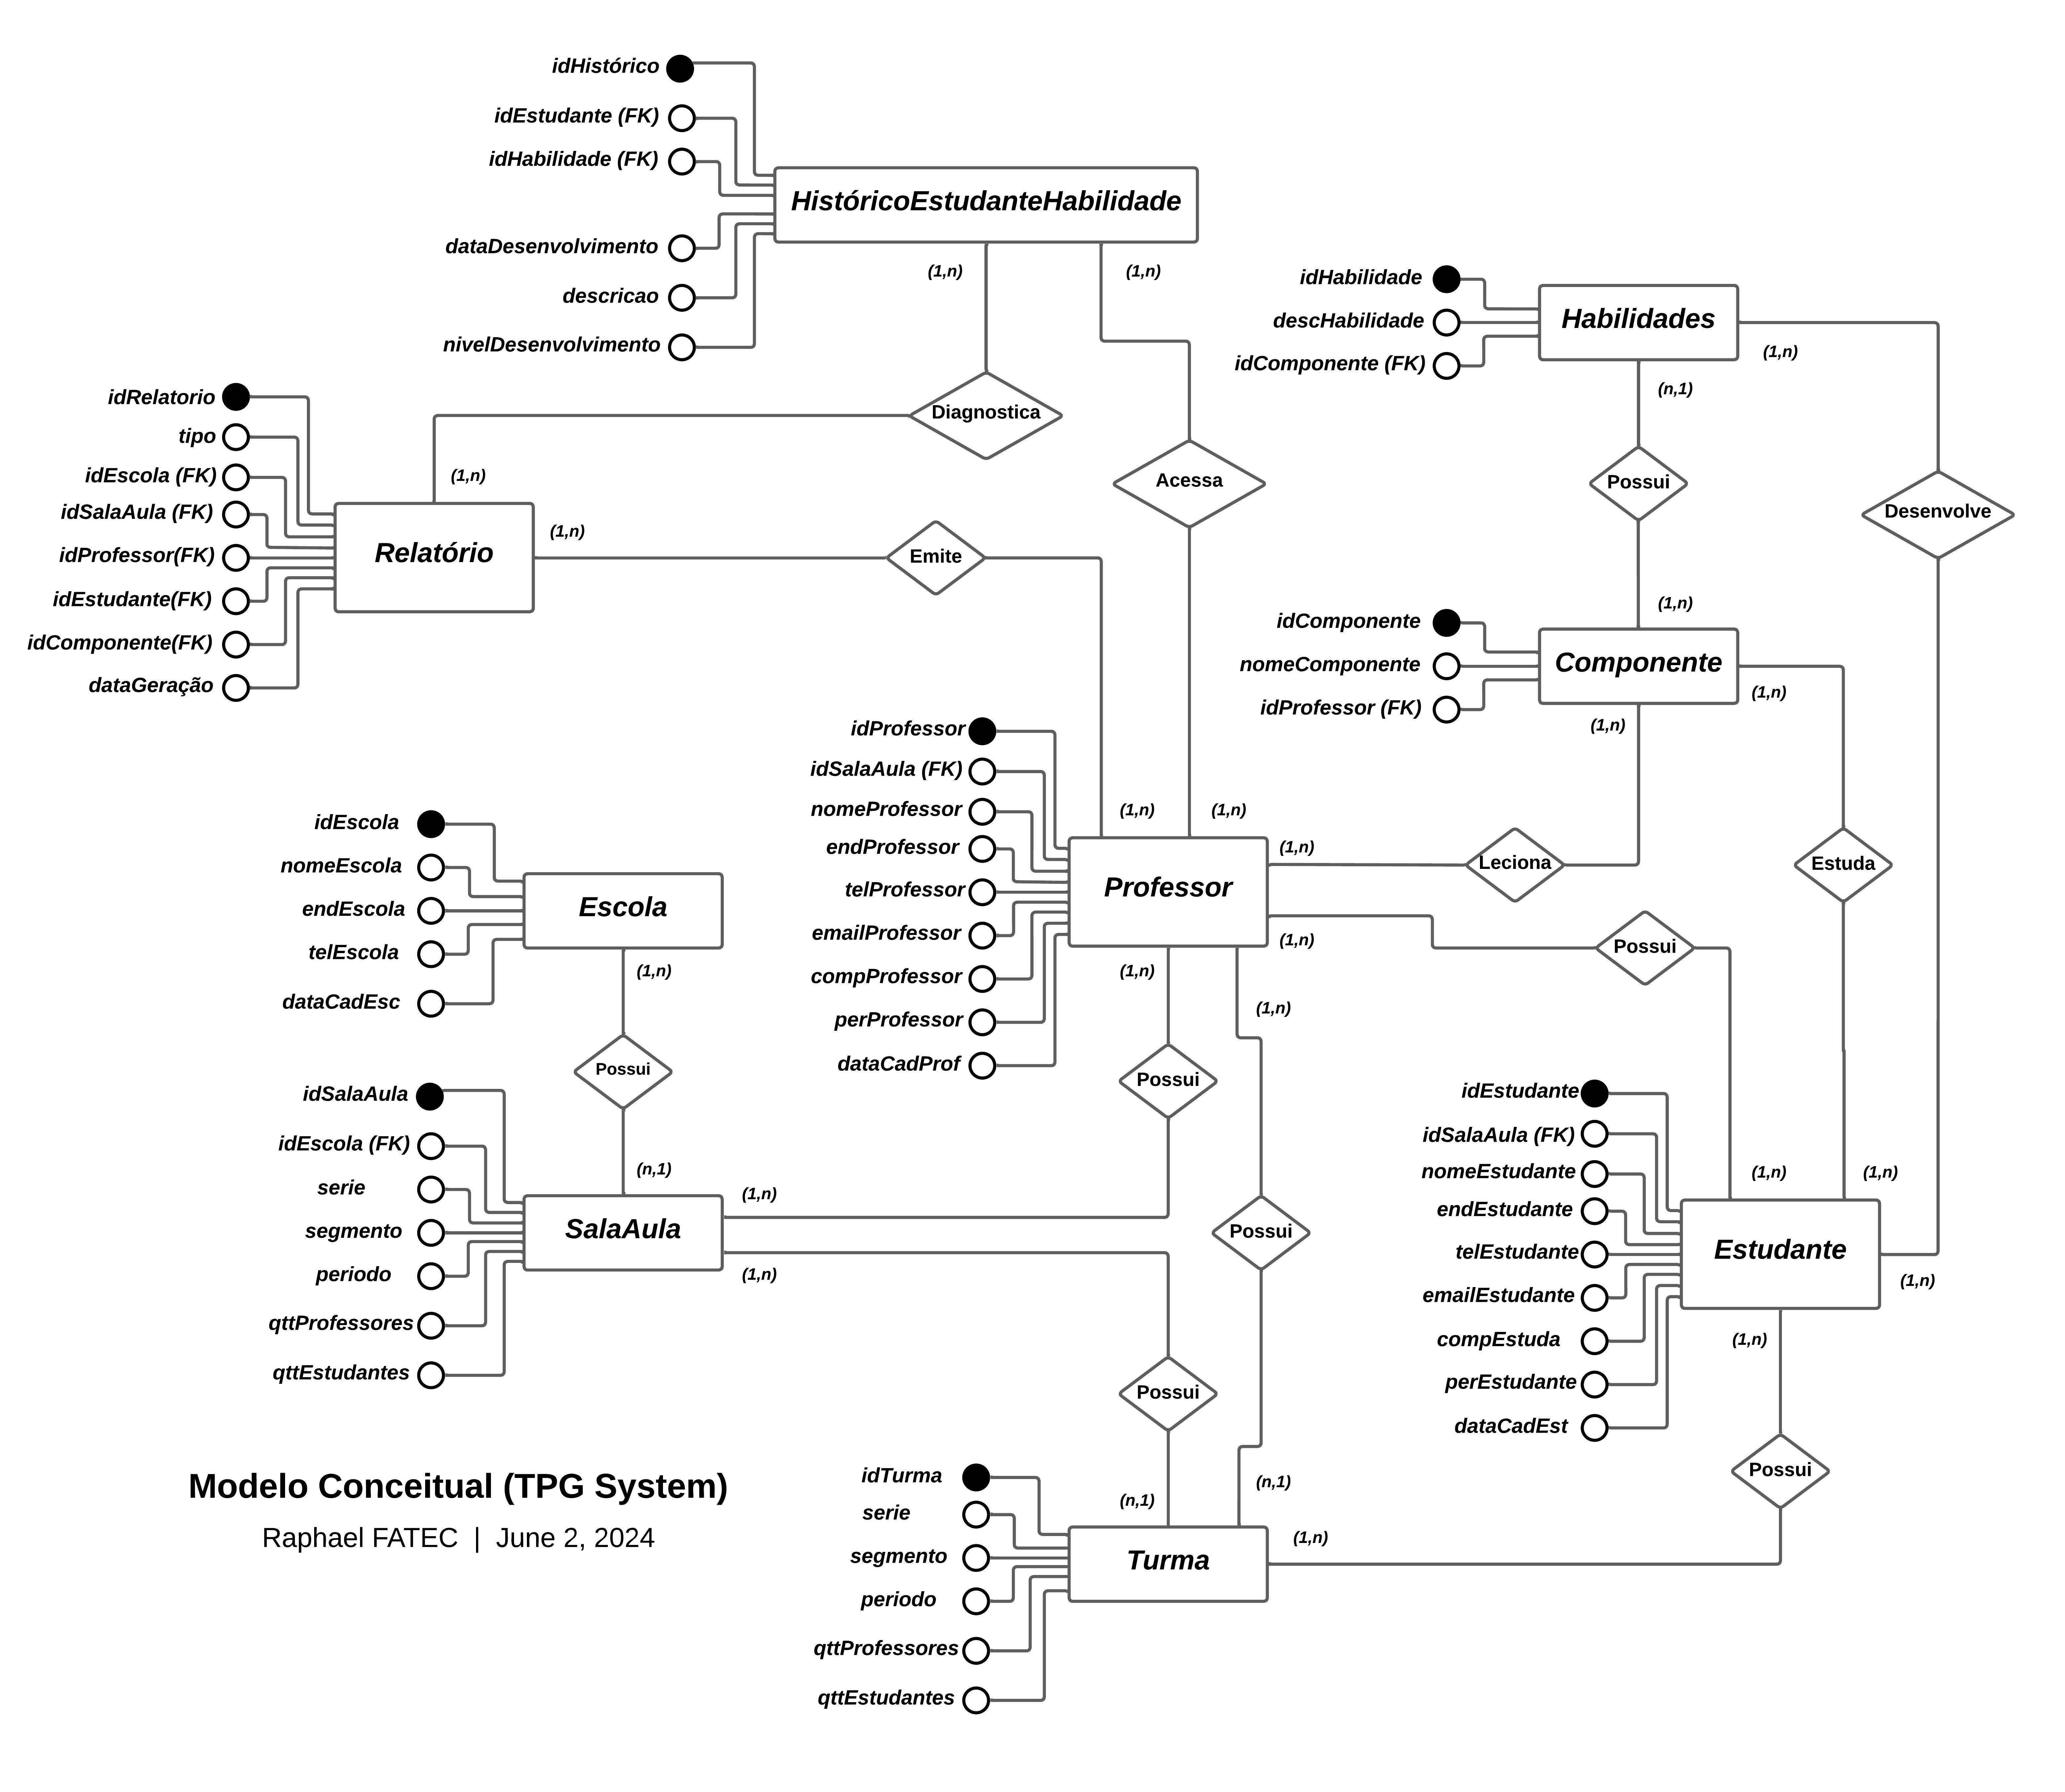
\includegraphics[scale=0.34]{Illustrations/imgdgMC.jpg}
\SourceOrNote{Autoria Própria (2024)}
\end{flowchart}
\\
\pagebreak

\begin{flowchart}[!h]
\centering
\caption{Diagrama de Modelagem Lógica - TPG System}%
\label{fcht:imgdgML.jpg}
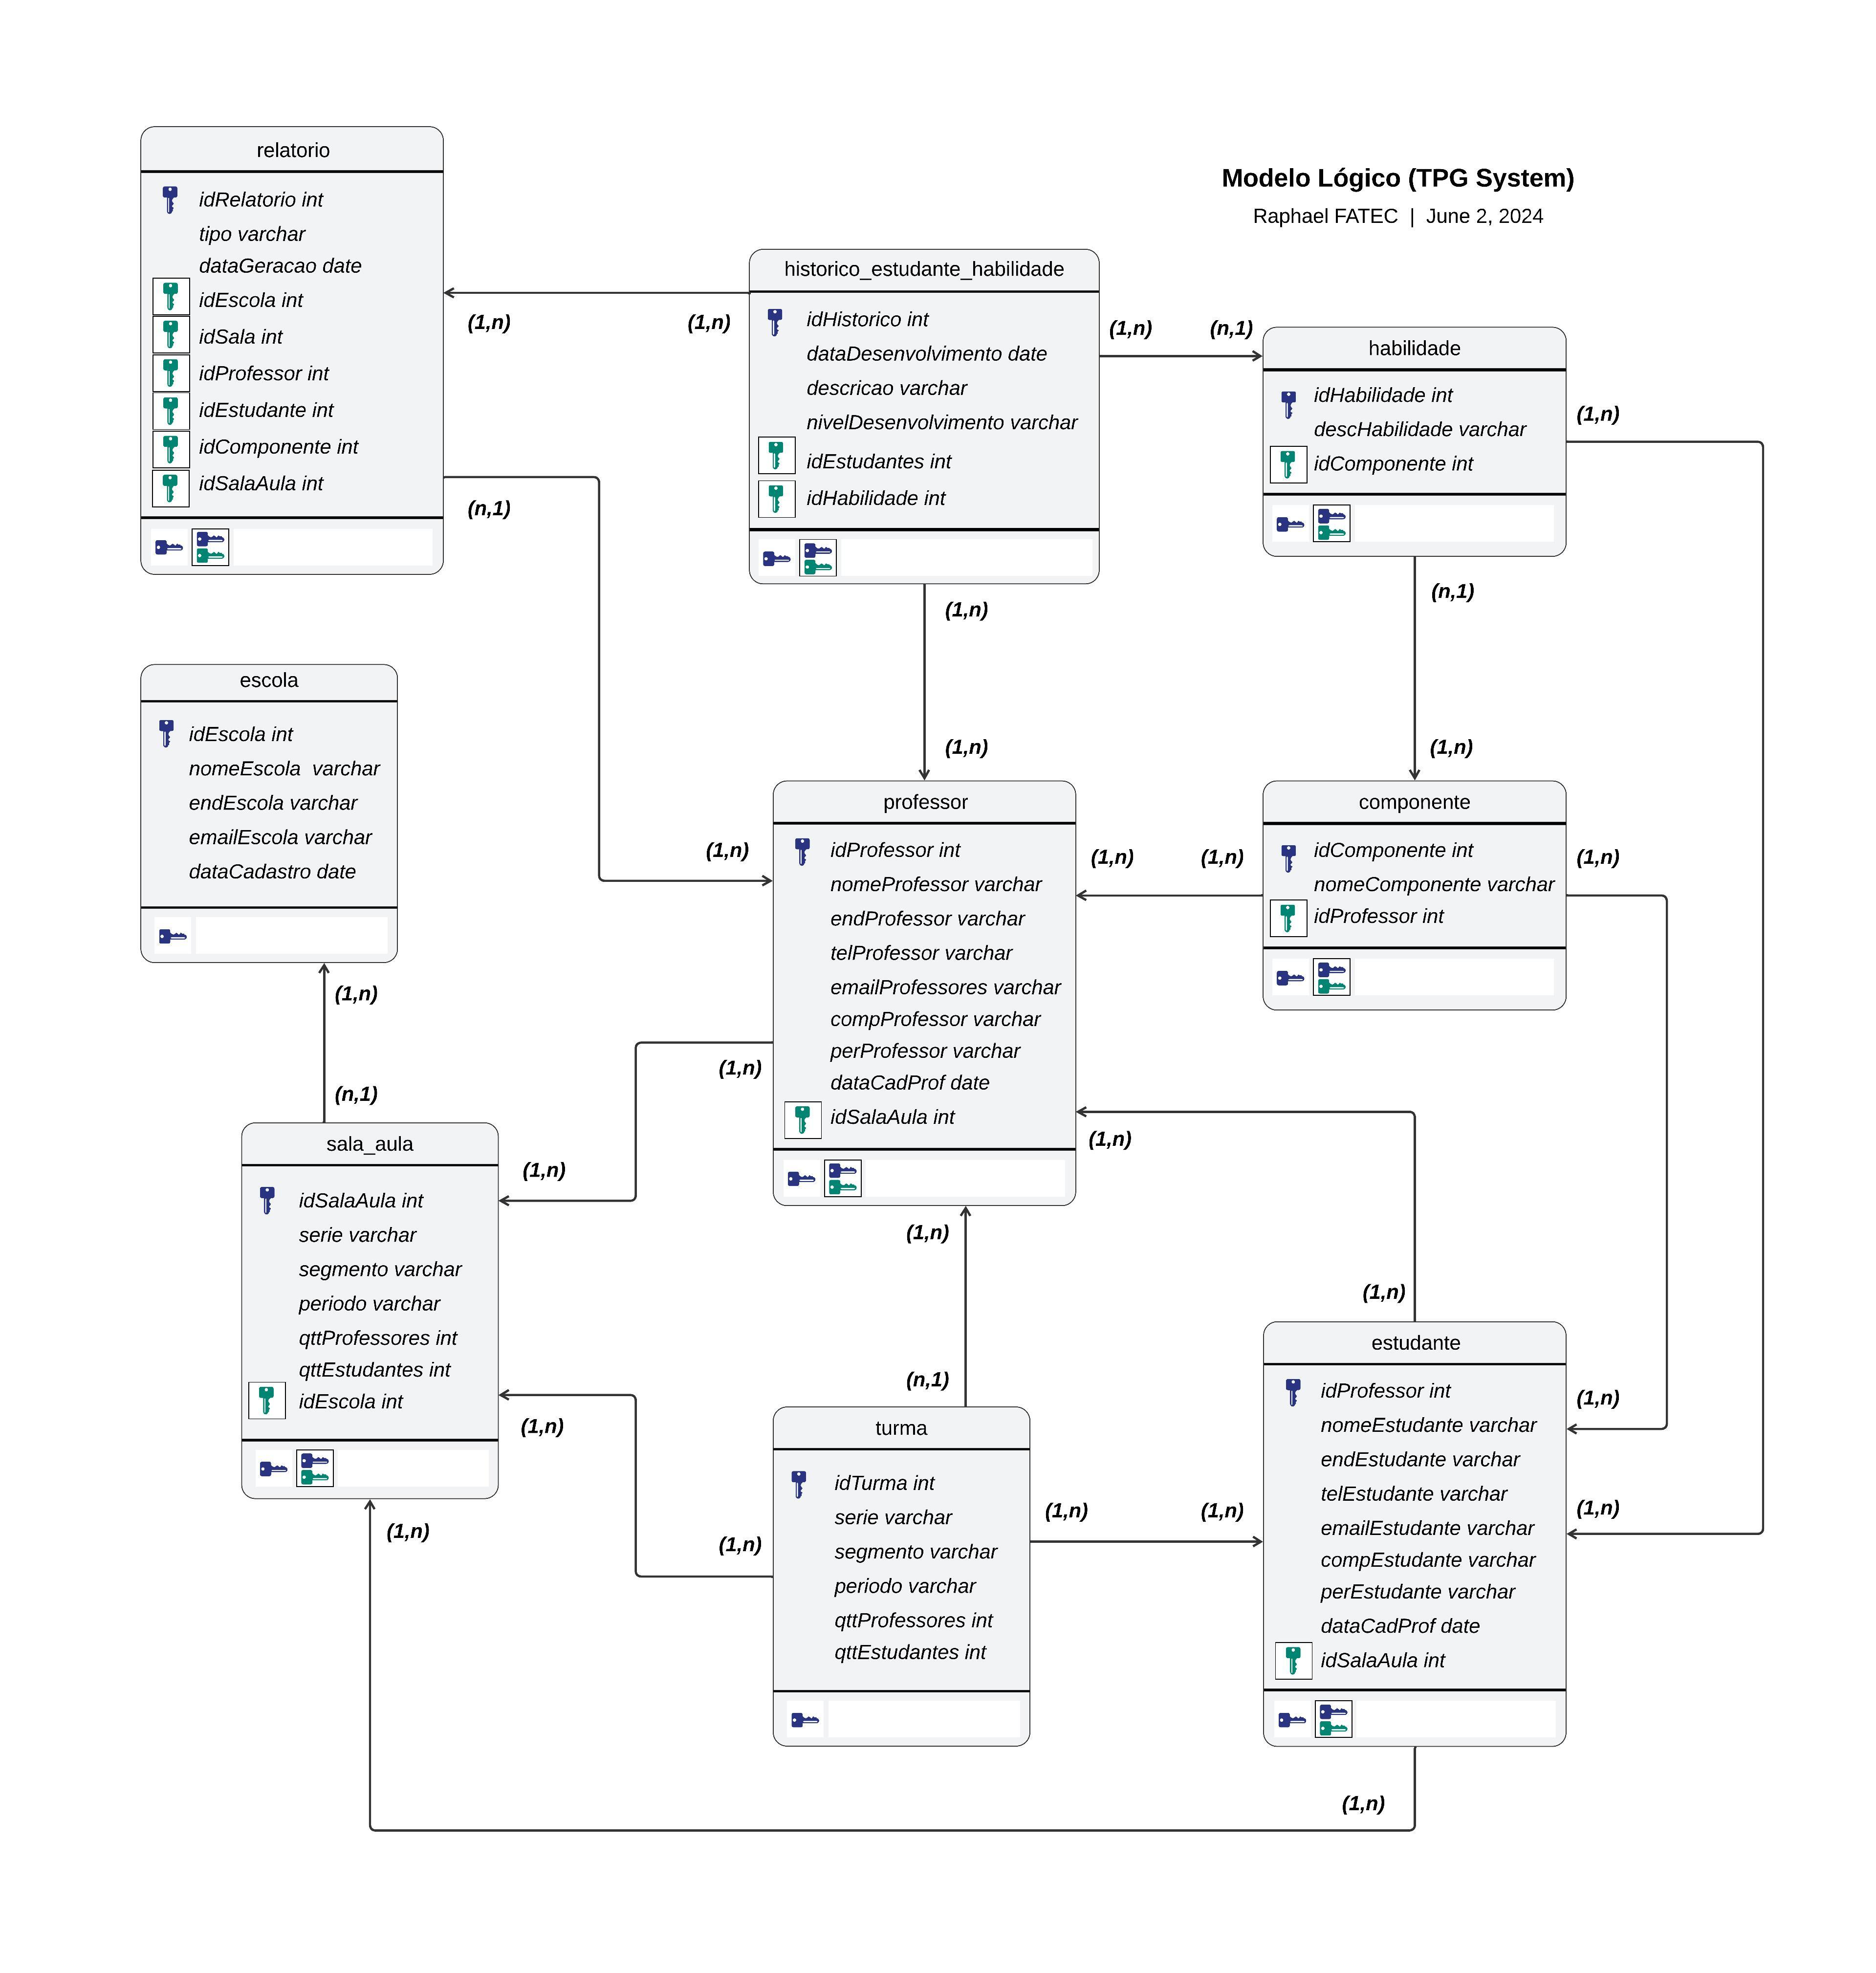
\includegraphics[scale=0.55]{Illustrations/imgdgML.jpg}
\SourceOrNote{Autoria Própria (2024)}
\end{flowchart}

\begin{itemize}

\item \textbf{Diagramas de Classe e Objeto:}
\\

\end{itemize}

No Diagrama de Classes do TPG System (\Cref{fcht:imgdgC.jpg}), podem-se observar diversas classes e seus relacionamentos, detalhando a estrutura de um sistema educacional com componentes curriculares, professores, alunos e desafios.
\\

\begin{flowchart}[!h]
\centering
\caption{Diagrama de Classe - TPG System}%
\label{fcht:imgdgC.jpg}
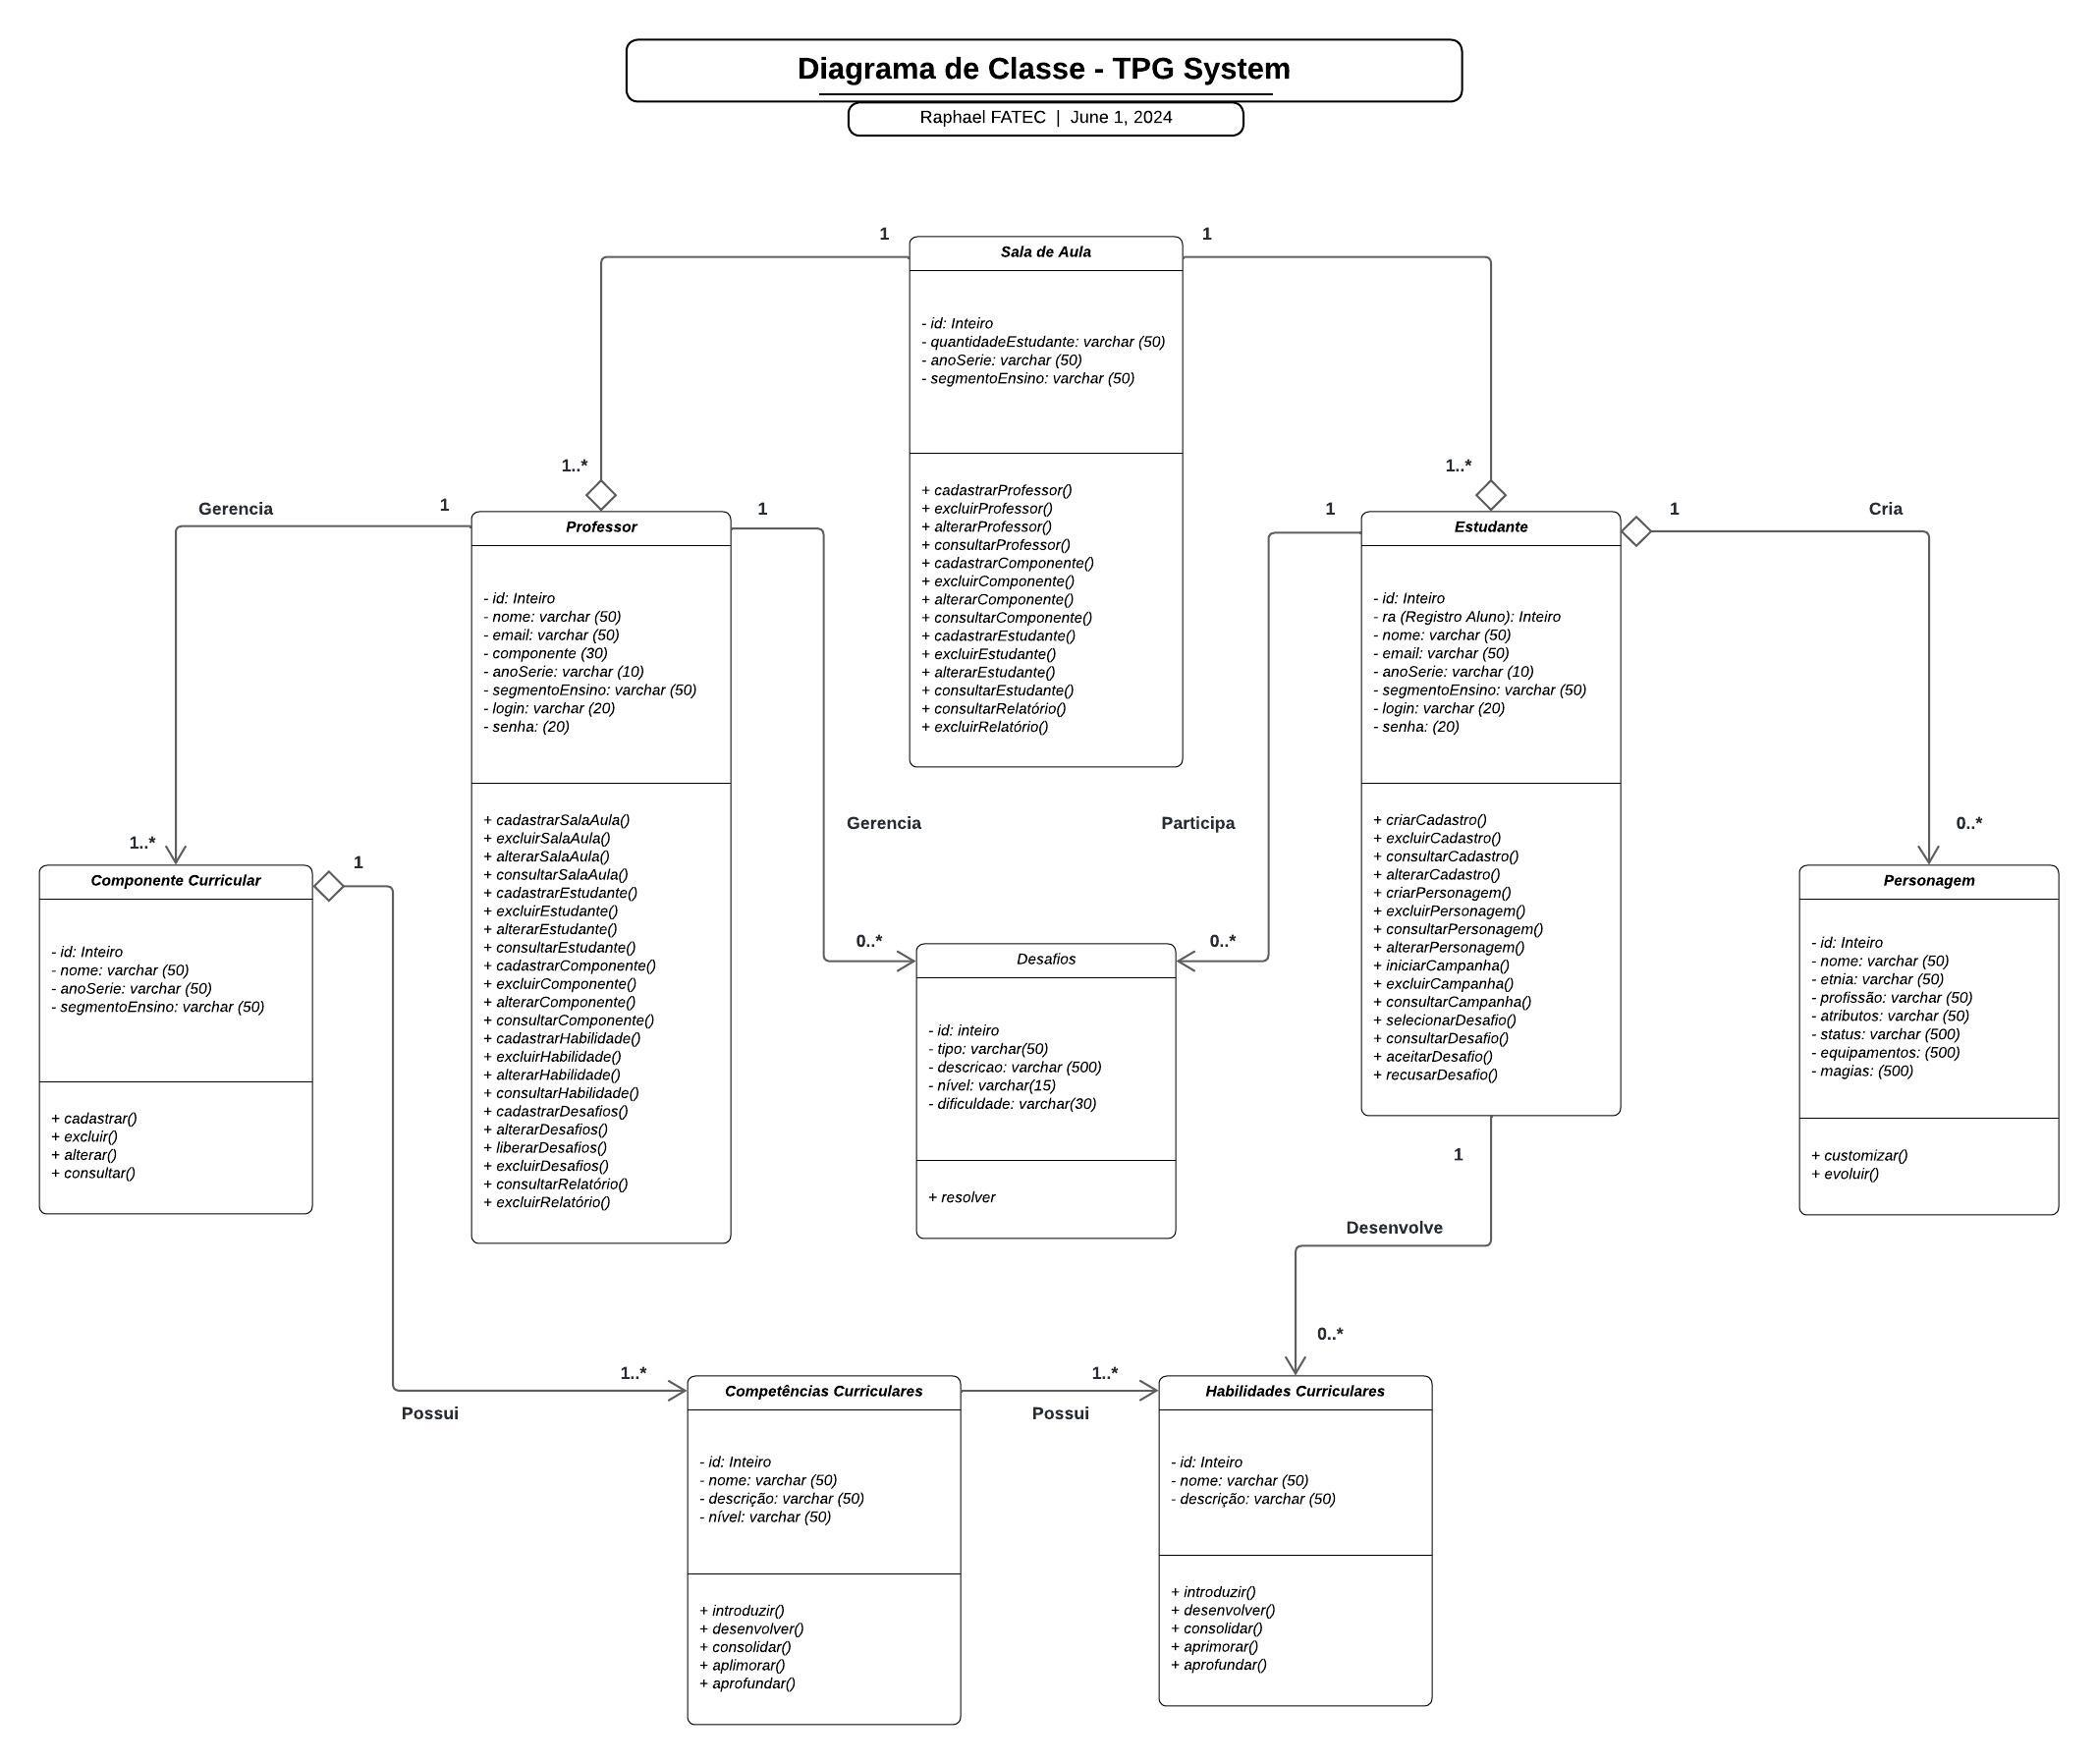
\includegraphics[scale=0.47]{Illustrations/imgdgC.jpg}
\SourceOrNote{Autoria Própria (2024)}
\end{flowchart}

Esse diagrama fornece uma visão abrangente da estrutura e dos relacionamentos essenciais para o funcionamento do sistema. Ao detalhar as classes, seus atributos e métodos, além das interações entre elas, o diagrama facilita a compreensão e a comunicação entre os desenvolvedores e outras partes interessadas, servindo como uma ferramenta de planejamento fundamental para a arquitetura do software.
\\

Nos Diagramas de Objetos, é apresentado o percurso do Professor (\Cref{fcht:imgdgObP.jpg}), detalhando o processo de cadastro e acesso sistêmico, bem como a importância de ter acesso aos recursos específicos do sistema. Isso permite que as informações necessárias possam ser incluídas, alteradas e consultadas de forma dinâmica e ordenada.
\\

\begin{flowchart}[!h]
\centering
\caption{Diagrama de Objeto (Professor) - TPG System}%
\label{fcht:imgdgObP.jpg}
\includegraphics[scale=0.50]{Illustrations/imgdgObP.jpeg}
\SourceOrNote{Autoria Própria (2024)}
\end{flowchart}

Quanto ao percurso do Estudante (\Cref{fcht:imgdgObE.jpg}), embora seja um caminho menos complexo no quesito de alimentação do sistema, pois ele já estará interagindo com as informações previamente inseridas pelo professor, exige um cuidado significativo para armazenar os dados de retorno. Isso é fundamental para subsidiar o sistema, permitindo a consulta, ordenação e geração de relatórios para o professor.
\\

\begin{flowchart}[!h]
\centering
\caption{Diagrama de Objeto (Estudante) - TPG System}%
\label{fcht:imgdgObE.jpg}
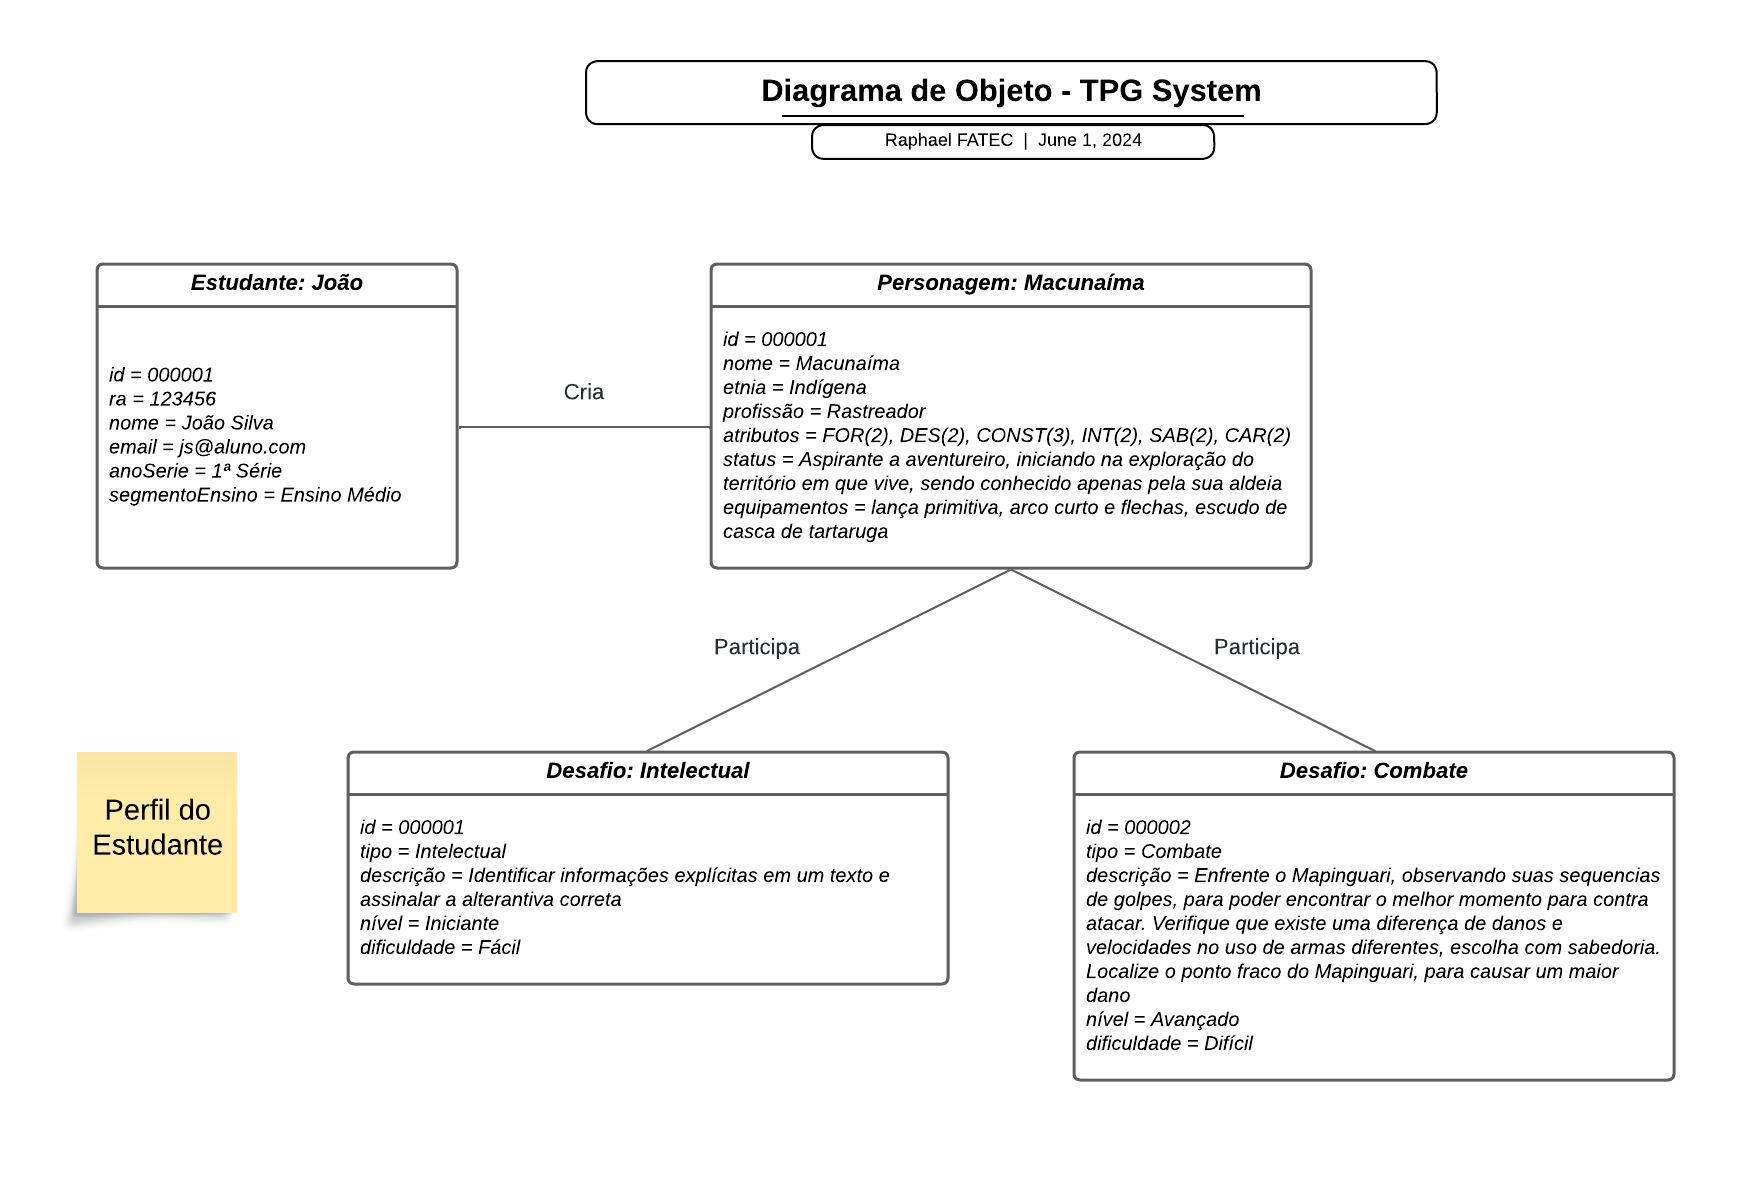
\includegraphics[scale=0.40]{Illustrations/imgdgObE.jpg}
\SourceOrNote{Autoria Própria (2024)}
\end{flowchart}

Esses diagramas fornecem exemplos concretos de como as classes e suas relações se manifestam em instâncias específicas dentro do sistema TPG. Eles ajudam a visualizar a estrutura do sistema educacional, mostrando como estudantes, professores, personagens e desafios interagem de maneira prática, facilitando o planejamento e desenvolvimento do software educacional
\\

\begin{itemize}

\item \textbf{Caso de Uso:}
\\

\end{itemize}


O processo de verificação e permissões no sistema resultou na estruturação do Caso de Uso em dois fluxogramas: o primeiro apresenta o Perfil do Professor (\Cref{fcht:imgdgCuP.jpg}), no qual é essencial o cadastro da Sala de Aula (representado em azul), ao qual o professor está vinculado, para a liberação do cadastro e acesso dos estudantes (representados em verde). Além disso, são fornecidas informações pertinentes sobre os Componentes que o professor leciona (representados em lilás), bem como a possibilidade de gerar os Relatórios Pedagógicos e acompanhar a evolução e/ou defasagem dos estudantes (representados em amarelo). É importante ressaltar que este fluxo deve ocorrer antes do cadastro pelos estudantes no sistema, visando facilitar a vinculação e cruzamento das informações.
\\

\begin{flowchart}[!h]
\centering
\caption{Diagrama de Caso de Uso - Perfil Professor - TPG System}%
\label{fcht:imgdgCuP.jpg}
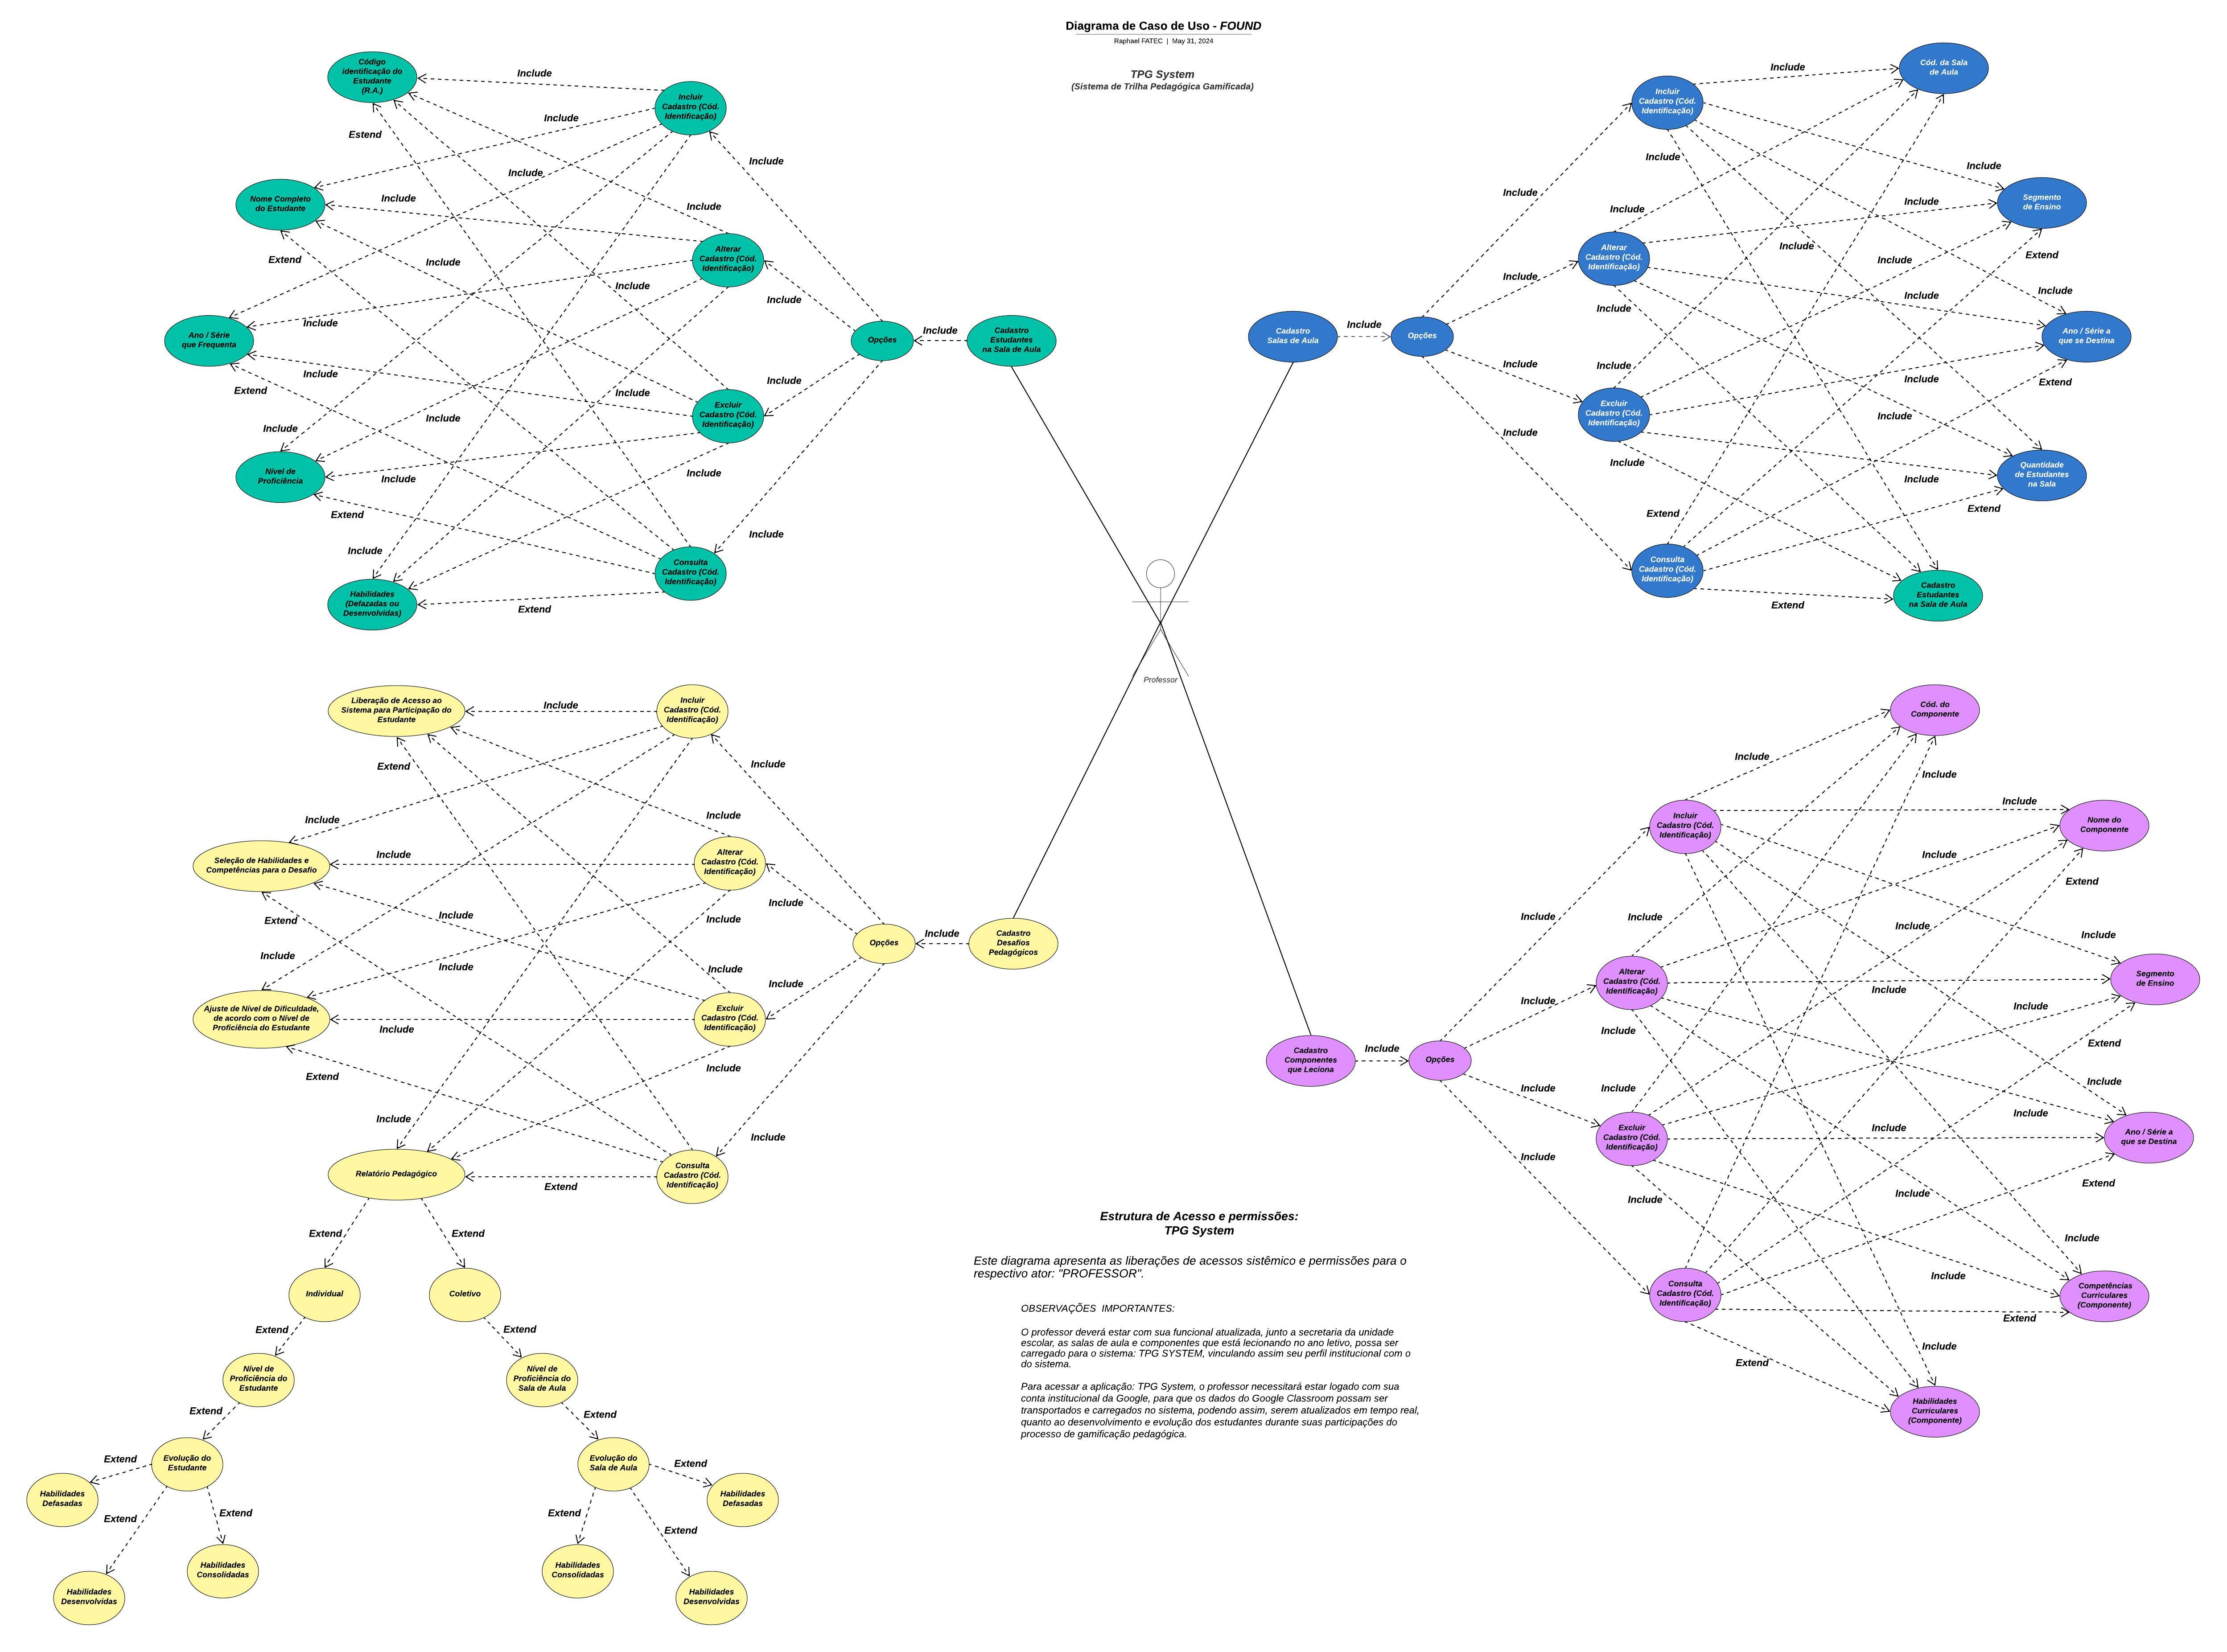
\includegraphics[scale=0.23]{Illustrations/imgdgCuP.jpg}
\SourceOrNote{Autoria Própria (2024)}
\end{flowchart}

Pelo Perfil do Estudante (\Cref{fcht:imgdgCuE.jpg}), nota-se que ele possui acesso interno ao sistema, podendo realizar a Criação de Seu Personagem (representado em azul claro) e iniciar propriamente o processo de participação efetiva no Sistema Pedagógico Gamificado, interagindo diretamente com a interface do sistema.
\\

\begin{flowchart}[!h]
\centering
\caption{Diagrama de Caso de Uso - Perfil Estudante - TPG System}%
\label{fcht:imgdgCuE.jpg}
\includegraphics[scale=0.33]{Illustrations/imgdgCuE.jpg}
\SourceOrNote{Autoria Própria (2024)}
\end{flowchart}

Dessa forma, pode-se inferir que o Professor atua mais como observador e mediador do processo, enquanto o verdadeiro protagonista é o Estudante. Entretanto, é importante ressaltar que os desafios e os níveis de dificuldade são estruturados pelo próprio sistema, com base nas informações fornecidas previamente pelo professor referentes às habilidades e competências do Componente Curricular. Isso possibilita que tais desafios sejam ofertados aos estudantes de forma adequada.
\\

Além disso, com base nas respostas dadas pelos estudantes, o sistema consegue estruturar os relatórios necessários para que o professor melhore suas estratégias pedagógicas e metodologias na sala de aula. Esses relatórios fornecem insights valiosos sobre o desempenho individual e coletivo dos alunos, permitindo ao professor ajustar suas abordagens de ensino de acordo com as necessidades identificadas.
\\

\begin{itemize}

\item \textbf{Diagrama de Rede:}
\\

\end{itemize}

O Diagrama de Rede (\Cref{fcht:dgR.jpg}), representa graficamente a estrutura, as atividades, dependências e o fluxo de trabalho do projeto. Esta ferramenta é fundamental no gerenciamento de projetos e oferece os seguintes benefícios:
\\

\begin{flowchart}[!h]
\centering
\caption{Diagrama de Rede - TPG System}%
\label{fcht:dgR.jpg}
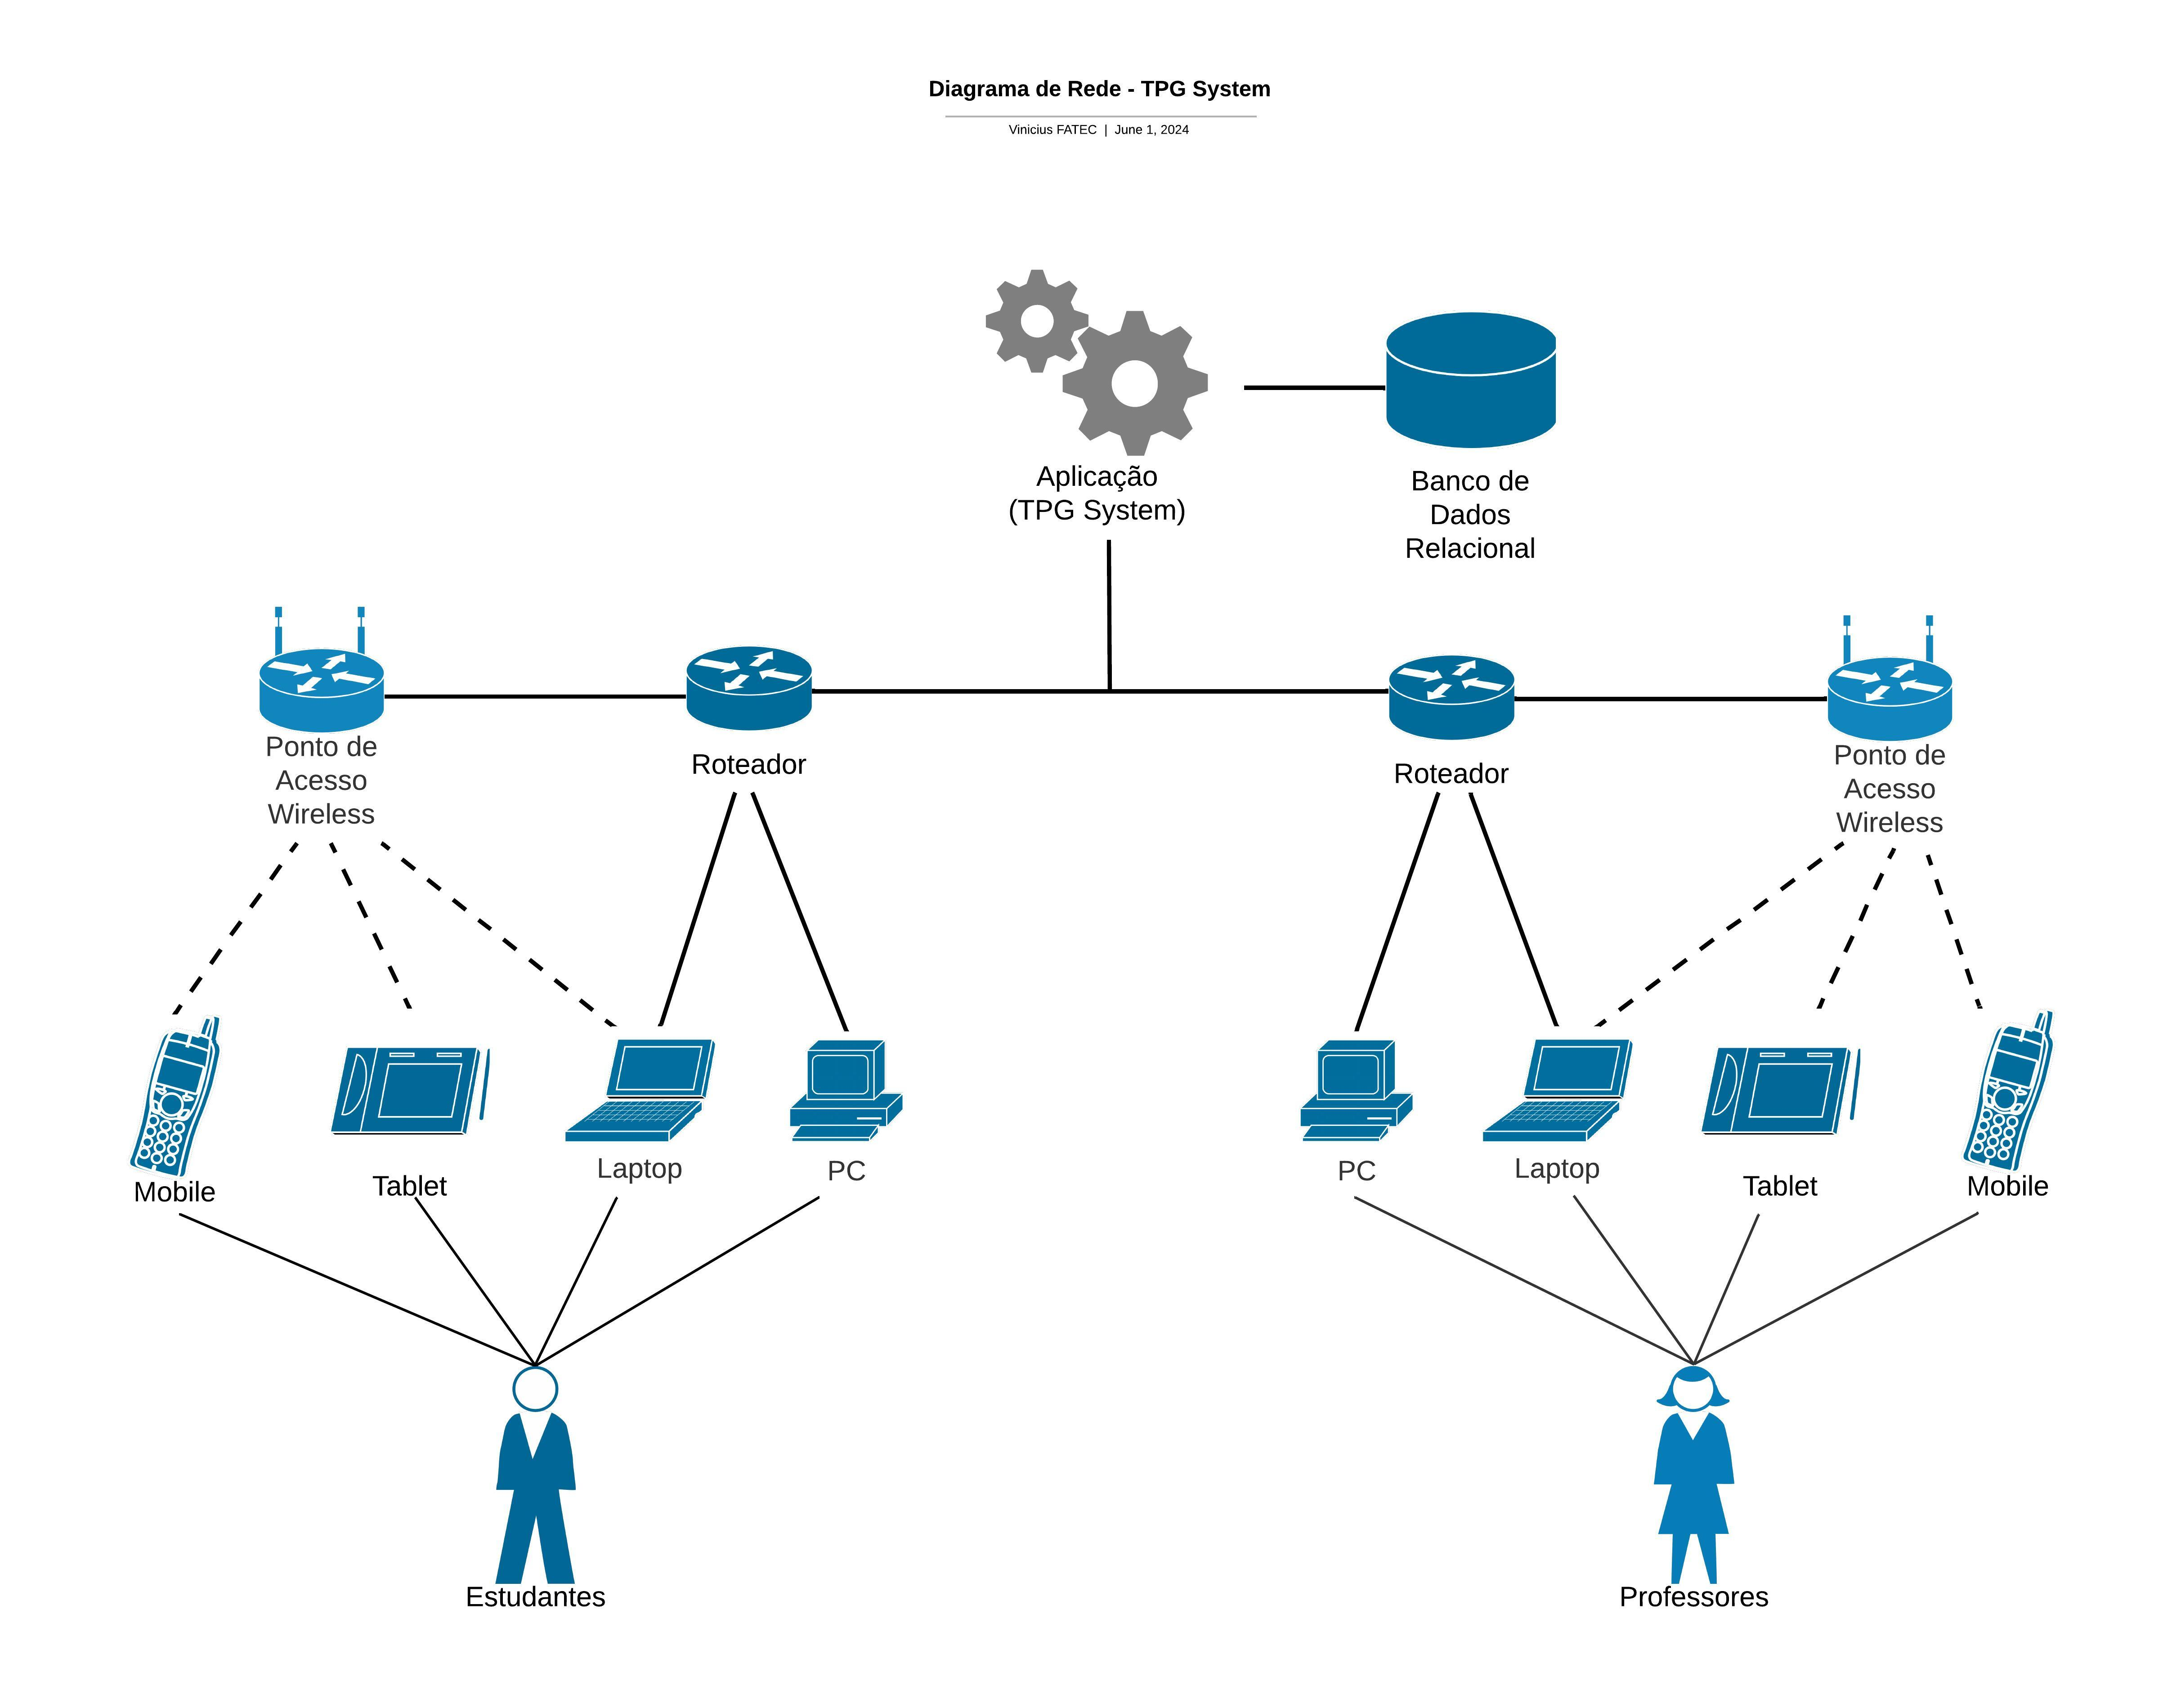
\includegraphics[scale=0.32]{Illustrations/dgR.jpg}
\SourceOrNote{Autoria Própria (2024)}
\end{flowchart}

\\
\begin{enumerate}
\item \textbf{Visualização das Atividades e Dependências:} Ajuda a visualizar todas as tarefas necessárias para a conclusão do projeto, bem como suas interdependências. Isso facilita a compreensão de como as atividades se relacionam e se influenciam mutuamente;  
\\ 
\item \textbf{Planejamento e Sequenciamento: } Permite identificar a sequência lógica das atividades, o que é crucial para o planejamento eficiente do cronograma do projeto;
\\
\item \textbf{Identificação do Caminho Crítico:} O diagrama ajuda a identificar o caminho crítico, ou seja, a sequência de atividades que determina a duração total do projeto. Isso é vital para gerenciar prazos e garantir que o projeto seja concluído no tempo estimado; 
\\
\item \textbf{Gestão de Recursos:} Facilita a alocação e o gerenciamento de recursos, identificando onde e quando recursos específicos serão necessários;  
\\ 
\item \textbf{Análise de Riscos e Problemas:} Permite uma análise mais detalhada de possíveis riscos e gargalos no projeto, ajudando a antecipar e mitigar problemas antes que eles ocorram;
\\
\item \textbf{Comunicação e Colaboração:} Serve como uma ferramenta de comunicação eficiente entre membros da equipe e partes interessadas, promovendo uma melhor colaboração e entendimento compartilhado do progresso do projeto; 
\\
\end{enumerate}

\begin{itemize}

\item \textbf{Análise de implementação de algoritmos de ordenação e sua eficácia na aplicação:}
\\

\end{itemize}

Ao considerar várias situações hipotéticas, a mais crítica é o desenvolvimento de um relatório pedagógico que mostre a realidade cotidiana. Com base nesse apontamento, pensou-se no seguinte cenário:
\\

Uma unidade escolar com 7 salas de aula, sendo uma de cada ano/série (6º ano, 7º ano, 8º ano, 9º ano, 1ª série EM, 2ª série EM, 3ª série EM), contendo em média 40 estudantes regularmente matriculados e frequentes. Cada sala de aula possui em média 12 professores, correspondendo a 12 componentes curriculares. Um componente curricular possui em média 30 habilidades. Um professor necessita retirar um relatório pedagógico, em ordem decrescente, contendo todos os estudantes que mais desenvolveram habilidades (\Cref{fig:MergeSort.jpg}).
\\
\begin{figure}[!h]
\centering
\caption{Algorítimo de Ordenação: MergeSort - TPG System}%
\label{fig:MergeSort.jpg}
\includegraphics[scale=0.42]{Illustrations/MergeSort.jpg}
\SourceOrNote{Autoria Própria (2024)}
\end{figure}

O algoritmo de ordenação Merge Sort apresenta um desempenho consistente e garante uma complexidade de tempo de O(n log n), além de manter a estabilidade, preservando a ordem relativa dos elementos iguais. Embora exija espaço adicional de memória para criar arrays auxiliares durante a mesclagem, sua vantagem reside na facilidade de implementação em comparação com o QuickSort. Para este teste, que não envolve uma quantidade moderada de dados e não foram mencionadas preocupações com estabilidade ou restrições de memória, o QuickSort poderia ser uma escolha razoável. Este método normalmente oferece um desempenho rápido e é amplamente empregado em diversos cenários. No entanto, por trabalharmos em um ambiente real com grande fluxo de dados e a necessidade de estabilidade no processo, ou a garantia de desempenho no pior caso forem preocupações importantes, o MergeSort se torna a opção mais segura.





\section*{CONCLUSÃO}\label{sect:conclusao}

Com base nos apontamentos apresentados, a situação problema reside na busca por estratégias inovadoras e eficazes que promovam um aprendizado mais significativo e inclusivo no contexto educacional. Diante desse desafio, propõe-se a implementação de uma Trilha Pedagógica Gamificada com elementos de Role-Playing Game (RPG), que integra Metodologias Ativas de Aprendizagem. Essa abordagem visa engajar os estudantes, desenvolver habilidades e competências, e promover a construção interdisciplinar do conhecimento, alinhando-se às diretrizes curriculares nacionais e aos objetivos de uma educação integral.
\\

A proposta de solução abrange a criação de um Sistema de Trilha Pedagógica Gamificada com Elementos de RPG, aplicável em diversos contextos educacionais. Esse sistema facilitará o monitoramento e a tomada de decisões pelos docentes, promovendo uma educação mais personalizada e envolvente. Para tanto, serão desenvolvidos protótipos de interface no Figma, planejado o modelo de negócios com o Business Model Canvas, modelado o sistema de software com a UML e o DER, e estruturado o banco de dados com XAMPP e MySQL. O desenvolvimento do sistema ocorrerá no Visual Studio Code com Node.js, e os personagens serão criados na plataforma Hero Forge.
\\

O desenvolvimento meticuloso da aplicação representa um avanço significativo na integração da tecnologia e metodologias ativas de aprendizagem. Além de oferecer uma oportunidade para repensar e revitalizar o processo educacional, essa iniciativa capacita educadores e estudantes com uma ferramenta poderosa que pode catalisar a transformação do ensino e da aprendizagem. Ao fornecer uma interface intuitiva, um sistema de recompensas motivador e uma estrutura flexível, está se construindo as bases para um sistema educacional mais inclusivo, adaptável e eficaz.
\\

Portanto, o desenvolvimento minucioso e cuidadoso dessa aplicação é fundamental para o futuro da educação. Ao oferecer ferramentas e recursos inovadores que capacitam educadores e engajam os estudantes de maneira mais profunda e significativa, está-se dando passos importantes em direção a uma educação mais alinhada com as demandas do século XXI. A aplicação da Trilha Pedagógica Gamificada com Elementos de RPG representa um marco na evolução da prática educacional, promovendo um ambiente de aprendizado dinâmico, envolvente e adaptado às necessidades individuais dos estudantes.
\\












\printbibliography

%% Elementos pós-textuais (opcionais): Apêndice e Anexo
%Caso for utilizar, basta retirar o símbolo de % na frente do comando
%%%%% Elementos pós-textuais
%%
%% Glossário, apêndices, anexos e índice remissivo (opcionais).

%% Apêndices
\begin{Appendix}

\section{Título de Apêndice}%
\label{sect:apx-a1}

Exemplo de apêndice (\Cref{sect:apx-a1}) em uma seção de \nameref{sect:appendix}.

\subsection{Título de Seção Secundária de Apêndice}%
\label{ssect:apx-a2}

Exemplo de seção secundária de apêndice (\Cref{ssect:apx-a2}).

\subsubsection{Título de Seção Terciária de Apêndice}%
\label{sssect:apx-a3}

Exemplo de seção terciária de apêndice (\Cref{sssect:apx-a3}).

\paragraph{Título de seção quaternária de Apêndice}%
\label{prgh:apx-a4}

Exemplo de seção quaternária de apêndice (\Cref{prgh:apx-a4}).

\subparagraph{Título de seção quinária de Apêndice}%
\label{sprgh:apx-a5}

Exemplo de seção quinária de apêndice (\Cref{sprgh:apx-a5}).

\end{Appendix}

%% Anexos
\begin{Annex}

\section{Título de Anexo}%
\label{sect:anx-a1}

Exemplo de anexo (\Cref{sect:anx-a1}) em uma seção de \nameref{sect:annex}.

\subsection{Título de Seção Secundária de Anexo}%
\label{ssect:anx-a2}

Exemplo de seção secundária de anexo (\Cref{ssect:anx-a2}).

\subsubsection{Título de Seção Terciária de Anexo}%
\label{sssect:anx-a3}

Exemplo de seção terciária de anexo (\Cref{sssect:anx-a3}).

\paragraph{Título de seção quaternária de Anexo}%
\label{prgh:anx-a4}

Exemplo de seção quaternária de anexo (\Cref{prgh:anx-a4}).

\subparagraph{Título de seção quinária de Anexo}%
\label{sprgh:anx-a5}

Exemplo de seção quinária de anexo (\Cref{sprgh:anx-a5}).

\end{Annex}

%% Índice remissivo
\printindex%

\\

%% Fim do documento
\end{document}